% Options for packages loaded elsewhere
\PassOptionsToPackage{unicode}{hyperref}
\PassOptionsToPackage{hyphens}{url}
\PassOptionsToPackage{dvipsnames,svgnames,x11names}{xcolor}
%
\documentclass[
  singlecolumn]{article}

\usepackage{amsmath,amssymb}
\usepackage{iftex}
\ifPDFTeX
  \usepackage[T1]{fontenc}
  \usepackage[utf8]{inputenc}
  \usepackage{textcomp} % provide euro and other symbols
\else % if luatex or xetex
  \usepackage{unicode-math}
  \defaultfontfeatures{Scale=MatchLowercase}
  \defaultfontfeatures[\rmfamily]{Ligatures=TeX,Scale=1}
\fi
\usepackage[]{libertinus}
\ifPDFTeX\else  
    % xetex/luatex font selection
\fi
% Use upquote if available, for straight quotes in verbatim environments
\IfFileExists{upquote.sty}{\usepackage{upquote}}{}
\IfFileExists{microtype.sty}{% use microtype if available
  \usepackage[]{microtype}
  \UseMicrotypeSet[protrusion]{basicmath} % disable protrusion for tt fonts
}{}
\makeatletter
\@ifundefined{KOMAClassName}{% if non-KOMA class
  \IfFileExists{parskip.sty}{%
    \usepackage{parskip}
  }{% else
    \setlength{\parindent}{0pt}
    \setlength{\parskip}{6pt plus 2pt minus 1pt}}
}{% if KOMA class
  \KOMAoptions{parskip=half}}
\makeatother
\usepackage{xcolor}
\usepackage[top=30mm,left=20mm,heightrounded]{geometry}
\setlength{\emergencystretch}{3em} % prevent overfull lines
\setcounter{secnumdepth}{-\maxdimen} % remove section numbering
% Make \paragraph and \subparagraph free-standing
\ifx\paragraph\undefined\else
  \let\oldparagraph\paragraph
  \renewcommand{\paragraph}[1]{\oldparagraph{#1}\mbox{}}
\fi
\ifx\subparagraph\undefined\else
  \let\oldsubparagraph\subparagraph
  \renewcommand{\subparagraph}[1]{\oldsubparagraph{#1}\mbox{}}
\fi


\providecommand{\tightlist}{%
  \setlength{\itemsep}{0pt}\setlength{\parskip}{0pt}}\usepackage{longtable,booktabs,array}
\usepackage{calc} % for calculating minipage widths
% Correct order of tables after \paragraph or \subparagraph
\usepackage{etoolbox}
\makeatletter
\patchcmd\longtable{\par}{\if@noskipsec\mbox{}\fi\par}{}{}
\makeatother
% Allow footnotes in longtable head/foot
\IfFileExists{footnotehyper.sty}{\usepackage{footnotehyper}}{\usepackage{footnote}}
\makesavenoteenv{longtable}
\usepackage{graphicx}
\makeatletter
\def\maxwidth{\ifdim\Gin@nat@width>\linewidth\linewidth\else\Gin@nat@width\fi}
\def\maxheight{\ifdim\Gin@nat@height>\textheight\textheight\else\Gin@nat@height\fi}
\makeatother
% Scale images if necessary, so that they will not overflow the page
% margins by default, and it is still possible to overwrite the defaults
% using explicit options in \includegraphics[width, height, ...]{}
\setkeys{Gin}{width=\maxwidth,height=\maxheight,keepaspectratio}
% Set default figure placement to htbp
\makeatletter
\def\fps@figure{htbp}
\makeatother
\newlength{\cslhangindent}
\setlength{\cslhangindent}{1.5em}
\newlength{\csllabelwidth}
\setlength{\csllabelwidth}{3em}
\newlength{\cslentryspacingunit} % times entry-spacing
\setlength{\cslentryspacingunit}{\parskip}
\newenvironment{CSLReferences}[2] % #1 hanging-ident, #2 entry spacing
 {% don't indent paragraphs
  \setlength{\parindent}{0pt}
  % turn on hanging indent if param 1 is 1
  \ifodd #1
  \let\oldpar\par
  \def\par{\hangindent=\cslhangindent\oldpar}
  \fi
  % set entry spacing
  \setlength{\parskip}{#2\cslentryspacingunit}
 }%
 {}
\usepackage{calc}
\newcommand{\CSLBlock}[1]{#1\hfill\break}
\newcommand{\CSLLeftMargin}[1]{\parbox[t]{\csllabelwidth}{#1}}
\newcommand{\CSLRightInline}[1]{\parbox[t]{\linewidth - \csllabelwidth}{#1}\break}
\newcommand{\CSLIndent}[1]{\hspace{\cslhangindent}#1}

\usepackage{cancel}
\usepackage[noblocks]{authblk}
\renewcommand*{\Authsep}{, }
\renewcommand*{\Authand}{, }
\renewcommand*{\Authands}{, }
\renewcommand\Affilfont{\small}
\usepackage{cancel}
\makeatletter
\makeatother
\makeatletter
\makeatother
\makeatletter
\@ifpackageloaded{caption}{}{\usepackage{caption}}
\AtBeginDocument{%
\ifdefined\contentsname
  \renewcommand*\contentsname{Table of contents}
\else
  \newcommand\contentsname{Table of contents}
\fi
\ifdefined\listfigurename
  \renewcommand*\listfigurename{List of Figures}
\else
  \newcommand\listfigurename{List of Figures}
\fi
\ifdefined\listtablename
  \renewcommand*\listtablename{List of Tables}
\else
  \newcommand\listtablename{List of Tables}
\fi
\ifdefined\figurename
  \renewcommand*\figurename{Figure}
\else
  \newcommand\figurename{Figure}
\fi
\ifdefined\tablename
  \renewcommand*\tablename{Table}
\else
  \newcommand\tablename{Table}
\fi
}
\@ifpackageloaded{float}{}{\usepackage{float}}
\floatstyle{ruled}
\@ifundefined{c@chapter}{\newfloat{codelisting}{h}{lop}}{\newfloat{codelisting}{h}{lop}[chapter]}
\floatname{codelisting}{Listing}
\newcommand*\listoflistings{\listof{codelisting}{List of Listings}}
\makeatother
\makeatletter
\@ifpackageloaded{caption}{}{\usepackage{caption}}
\@ifpackageloaded{subcaption}{}{\usepackage{subcaption}}
\makeatother
\makeatletter
\@ifpackageloaded{tcolorbox}{}{\usepackage[skins,breakable]{tcolorbox}}
\makeatother
\makeatletter
\@ifundefined{shadecolor}{\definecolor{shadecolor}{rgb}{.97, .97, .97}}
\makeatother
\makeatletter
\makeatother
\makeatletter
\makeatother
\ifLuaTeX
  \usepackage{selnolig}  % disable illegal ligatures
\fi
\IfFileExists{bookmark.sty}{\usepackage{bookmark}}{\usepackage{hyperref}}
\IfFileExists{xurl.sty}{\usepackage{xurl}}{} % add URL line breaks if available
\urlstyle{same} % disable monospaced font for URLs
\hypersetup{
  pdftitle={Effective Causal Diagrams for Evolutionary Human Science},
  pdfauthor={Joseph A. Bulbulia},
  pdfkeywords={DAGS, Causal
Inference, Confounding, History, Psychology, Panel},
  colorlinks=true,
  linkcolor={blue},
  filecolor={Maroon},
  citecolor={Blue},
  urlcolor={Blue},
  pdfcreator={LaTeX via pandoc}}

\title{Effective Causal Diagrams for Evolutionary Human Science}


  \author{Joseph A. Bulbulia}
            \affil{%
                  Victoria University of Wellington, New Zealand, School
                  of Psychology, Centre for Applied Cross-Cultural
                  Research
              }
      
\date{2023-07-27}
\begin{document}
\maketitle
\begin{abstract}
Causation inherently unfolds in time. However, quantifying causal
effects paradoxically relies on counterfactuals that never transpire.
Here, I show that by aligning a causal diagram's spatial structure with
temporal order and considering counterfactual identifiability
assumptions, the utility of the graph markedly improves. Part 1 revisits
three fundamental assumptions needed for estimating causal effects. Part
2 considers confounding and employs chronologically ordered causal
diagrams to clarify causal interaction, mediation, and longitudinal
growth. Part 3 demonstrates how time-structured diagrams offer practical
guidance for data collection and modelling. Part 4 applies causal
diagrams to selection bias in the context of a three-wave panel,
underlining the need for proper sampling, retention, and management of
missing data. Lastly, Part 5 uses chronologically ordered causal
diagrams to outline threats to causal estimation from measurement error,
with special attention to demands in comparative cultural research.
\end{abstract}
\ifdefined\Shaded\renewenvironment{Shaded}{\begin{tcolorbox}[breakable, frame hidden, enhanced, interior hidden, borderline west={3pt}{0pt}{shadecolor}, sharp corners, boxrule=0pt]}{\end{tcolorbox}}\fi

\hypertarget{introduction}{%
\subsection{Introduction}\label{introduction}}

Correlation is not causation. However, persistent confusion in the
analysis and reporting of correlations has limited scientific progress
across many human sciences. The direction of causation frequently runs
opposite to the direction of manifest correlations. This problem is
widely known. Nevertheless, many human scientists report manifest
correlations using hedging language. Making matters worse, widely
adopted strategies for confounding control fail
(\protect\hyperlink{ref-mcelreath2020}{McElreath 2020}), suggesting a
``causality crisis'' (\protect\hyperlink{ref-bulbulia2022}{J. A.
Bulbulia 2022}). Addressing the causality crisis is among the human
science's most pressing tasks.

When integrated into methodologically rigorous workflows, causal
Directed Acyclic Graphs (``DAGs'' or ``causal diagrams'') can be
powerful tools for clarifying causality.\footnote{The term ``DAG'' is
  unfortunate because not all directed acyclic graphs are causal. For a
  graph to be causal, it must satisfy the conditions of Markov
  factorisation (see: Part 2).} A system of formal mathematical proofs
underpins their design. This quality brings confidence. No formal
mathematical training is required to use them. This quality makes them
accessible. However, causal inference relies on assumptions. Causal
diagrams are methods for encoding such assumptions. Where assumptions
are unwarranted, causal diagrams may deceive. For example, when
researchers lack time-series data, unbiased causal effect estimates are
generally unwarranted. Thus, cross-sectional researchers who deploy
causal diagrams use them as scaffolding to uphold shaky assumptions.
Ideally, however, causal diagrams would serve as circuit breakers,
halting such misapplications in their tracks.

Here, I introduce a suite of techniques for constructing causal
diagrams. The core of this advice is to develop \emph{chronologically
ordered causal diagrams} -- that is, causal diagrams in which the
temporal order of cause and effect is evident in labelling and spatial
layout. I then illustrate the application of chronologically ordered
causal diagrams for research design in cultural evolutionary research.

There are many excellent introductions to causal diagrams
(\protect\hyperlink{ref-rohrer2018}{Rohrer 2018};
\protect\hyperlink{ref-hernuxe1n2023}{M. A. Hernán and Robins 2023a};
\protect\hyperlink{ref-cinelli2022}{Cinelli, Forney, and Pearl 2022};
\protect\hyperlink{ref-barrett2021}{Barrett 2021};
\protect\hyperlink{ref-mcelreath2020}{McElreath 2020};
\protect\hyperlink{ref-greenland1999}{Greenland, Pearl, and Robins
1999}; \protect\hyperlink{ref-suzuki2020}{Suzuki, Shinozaki, and
Yamamoto 2020}; \protect\hyperlink{ref-pearl2009}{Pearl
2009a}).\footnote{An excellent resource is Miguel Hernan's free online
  course, here:
  \url{https://pll.harvard.edu/course/causal-diagrams-draw-your-assumptions-your-conclusions}.}
One may reasonably ask whether another introduction adds clutter. The
approach I present here hopes to add value in five ways.

\textbf{Part 1} introduces the counterfactual framework for causal
inference as the appropriate theoretical setting for developing causal
diagrams. Here I review the three fundamental identification assumptions
required for causal inference..

\textbf{Part 2} discusses the four primary forms of confounding. Here, I
introduce chronologically ordered causal diagrams and describe their
utility. Focusing on temporal ordering brings clarity and direction for
data collection and modelling. Here, I show that chronologically ordered
causal diagrams clarify the topics of causal interaction, causal
mediation, and longitudinal growth modelling in settings of
treatment-confounder feedback.

\textbf{Part 3} discusses the advantages of collecting repeated measures
data for at least three waves, benefits that chronologically ordered
causal diagrams make evident. This discussion of the three-wave panel
provides practical guidance for cultural evolutionary researchers
interested in recording history to obtain a quantitative causal
understanding for their questions.

\textbf{Part 4} discusses selection bias in a three-wave panel. Here, I
use chronologically ordered causal diagrams to clarify the importance of
adequate sampling and longitudinal retention.

\textbf{Part 5}, uses causal diagrams to clarify four types of
measurement bias that arise when addressing causal questions. This
section will be particularly beneficial to researchers in comparative
cultural research, and to those employing composite scales.

Throughout, it is the application of chronologically ordered causal
diagrams in the setting of counterfactual data science that illuminates
both effective research strategies and their limitations.

\hypertarget{part-1.-the-three-fundamental-identifiability-assumptions-of-causal-inference}{%
\subsection{Part 1. The Three Fundamental Identifiability Assumptions of
Causal
Inference}\label{part-1.-the-three-fundamental-identifiability-assumptions-of-causal-inference}}

Before we can answer causal questions, we must understand how to ask
them (\protect\hyperlink{ref-hernuxe1n2016}{Miguel A. Hernán et al.
2016a}). In this section I review vital concepts and identification
assumptions.

\hypertarget{the-fundamental-problem-of-causal-inference}{%
\subsubsection{The fundamental problem of causal
inference}\label{the-fundamental-problem-of-causal-inference}}

We are entitled to claim that \(A\) causes \(Y\) if altering \(A\) would
have influenced the outcome of \(Y\)
(\protect\hyperlink{ref-hume1902}{Hume 1902};
\protect\hyperlink{ref-lewis1973}{Lewis 1973}). This claim requires
counterfactual reasoning. The causal effect is conceived as a contrast
between the world as it is, and the world as it could have been. Our
objective in ``causal inference'' is to quantify the magnitude of such
contrasts.

Consider an observed correlation between cultural beliefs in Big Gods
and social complexity. Suppose we hope to quantify the magnitude of the
causal effect of such beliefs. Denote beliefs in Big Gods, the
``exposure'' or ``treatment,'' by \(A\). Denote social complexity, the
outcome, by \(Y\). For now, assume the exposure, outcome, and the units
on which the exposures and outcomes are measured, ``cultures'', are
well-defined. (We will revisit these assumptions shortly.)

To evaluate causality for any individual culture, we must establish two
counterfactual or ``potential'' outcomes:

\begin{itemize}
\tightlist
\item
  \(Y_i(a = 1)\): The social complexity of culture \(i\) under belief in
  Big Gods. This outcome is counterfactual for each culture where
  \(A_i = 0\).
\item
  \(Y_i(a = 0)\): The social complexity of culture \(i\) without belief
  in Big Gods. This outcome is counterfactual for each culture where
  \(A_i = 1\).\footnote{The counterfactual outcome under exposure
    \(A = a\) can be denoted in several ways, such as \(Y(a)\),
    \(Y^{a}\), and \(Y_a\), with \(Y(a)\) being our chosen notation. For
    simplicity, we assume the exposures are exhaustive.}
\end{itemize}

We can define the causal effect of belief in Big Gods on social
complexity for a given culture as the difference between potential
outcomes \(Y_i(a)\) under \emph{each} exposure level, (\(A_i = 1\) and
\(A_i = 0\)).

\[
\text{Causal Effect of Belief in Big Gods}_i = Y_i(1) - Y_i(0) 
\]

To determine causality, then, we require a contrast between two states
of the world, one of which is inevitably counterfactual. The individual
causal effect is not identified in the data. This is known as ``the
fundamental problem of causal inference''
(\protect\hyperlink{ref-rubin1976}{Rubin 1976};
\protect\hyperlink{ref-holland1986}{Holland 1986}). It arises because
the observable data necessarily provide partial evidence. Inferring
counterfactual contrasts thus becomes a special, elusive, \emph{missing
data problem} (\protect\hyperlink{ref-westreich2015}{Westreich et al.
2015}; \protect\hyperlink{ref-edwards2015}{Edwards, Cole, and Westreich
2015}).

\hypertarget{causal-inference-is-an-approach-for-estimating-average-marginal-causal-effects}{%
\paragraph{Causal inference is an approach for estimating average
(marginal) causal
effects}\label{causal-inference-is-an-approach-for-estimating-average-marginal-causal-effects}}

Individual-level causal effects are typically unobservable. However, we
can use observable data to estimate average causal effects when certain
assumptions are satisfied. To obtain these effects on the difference
scale, we must compute a contrast in average outcomes (or equivalently,
the average of the differences in outcomes) from units exposed to
different treatment levels. In the case of a binary exposure, the
contrast is between the average difference (or equivalently, the
difference of the averages) (1) when all units are exposed to a certain
level of treatment and (2) when none are exposed.\footnote{Note that the
  difference in average expectations is equivalent to the average of the
  differences in expectations.}

On the difference scale, where \(a\) and \(a^*\) denote different levels
of treatment, the average treatment effect (ATE) is given by the
expression

\[
ATE = E[Y(a)] - E[Y(a^*)]
\]

However, we have just said that each unit may receive only one level of
the exposure \(A_i = a\) or \(A_i = a^*\). As such, individual-level
causal effects are generally not identifiable. Because the treatment
groups are composed of individual units, the treatment groups will also
contain missing observations. Where ``ATE'' denotes the average
treatment effect, the problem can be expressed

\[
ATE = \bigg(E[Y(1)|A = 1]_{\text{observed}} + E[Y(1)|A = 0]_{\text{unobserved}}\bigg) - \bigg(E[Y(0)|A = 0]_{\text{observed}}  + E[Y(0)|A = 1]_{\text{unobserved}}\bigg)
\]

Causal inference is a framework of assumptions and techniques used for
deriving causal contrasts from observed or observable data. This is why
I have called it ``counterfactual data science.'' It is grounded in the
three fundamental identification assumptions of causal inference. To
effectively use causal diagrams, it is essential to comprehend their
role within this broader framework.

\hypertarget{identification-assumption-1-causal-consistency}{%
\subsubsection{Identification Assumption 1: Causal
Consistency}\label{identification-assumption-1-causal-consistency}}

We need both observed and unobserved potential outcomes to evaluate the
average treatment effects (ATE). Our problem is that at least half the
observations we need are missing.

The causal consistency assumption plays a pivotal role in resolving this
distinct missing data issue. It serves as the key that unlocks a
quantitative understanding of the counterfactual outcomes. Let
\(Y_i^{observed}|A_i\) denote an individual's observed outcome in
response to treatment. Where the causal consistency assumption is
satisfied, we may derive counterfactual outcomes from the following rule

\[
Y_i^{observed}|A = 
\begin{cases} 
Y_i(~a^*) & \text{if } A_i = a* \\
Y_i(~a~) & \text{if } A_i = a
\end{cases}
\]

That is, where the causal consistency assumption is tenable, we say that
observed outcomes under each individual's realised exposure are equal to
that counterfactual outcome under the same exposure. This equivalence
still only gives us (at most) half of the counterfactual outcomes that
we need to compute causal contrasts. However, we could only compute
counterfacutal contrasts using data with a bridge from observations to
counterfactual outcomes. The counterfactual consistency assumption, when
satisfied, provides that bridge.

\textbf{Causal consistency assumes no interference}: We say that the
potential outcome for unit \(i\) under treatment \(a_i\) satisfies the
causal consistency assumption if the outcome is independent of the
treatment assignment of any other unit \(j\):

\[
Y_i(a_i, a_j) = Y_i(a_i, a'_j)
\]

for all \(a_j, a'_j\).

Violations of this condition can occur when there are dependencies in
the data. For example, the efficacy of a vaccine may typically depend on
the frequency of vaccination in the population, violating the
non-interference assumption (\protect\hyperlink{ref-ogburn2022}{Ogburn
et al. 2022}; \protect\hyperlink{ref-murray2021}{Murray, Marshall, and
Buchanan 2021a}, \protect\hyperlink{ref-murray2021a}{2021b})

\textbf{The causal consistency assumption does not strictly require
homogeneity of treatment administrations}: under the theory of causal
inference under multiple exposures, where there are \(K\) different
versions of treatment \(A\), we may consistently estimate causal effects
under the assumptions of ``treatment variation irrelevance.'' We may
claim such an entitlement to the causal consistency assumption if the
effects of the variations of the treatment are independent of the
counterfactual outcomes under such treatments, that is, if there is no
confounding for \(K\)'s effect on \(Y\) given measured confounders \(L\)
such that

\[
K \coprod Y(k) | L
\]

or equivalently

\[
Y(k) \coprod K | L
\]

According to the theory of causal inference under multiple versions of
treatment, \(A\) functions as a ``coarsened indicator'' to estimate the
causal effect of the multiple versions of treatment \(K\) on \(Y(k)\)
(\protect\hyperlink{ref-vanderweele2009}{Tyler J. VanderWeele 2009},
\protect\hyperlink{ref-vanderweele2018}{2018};
\protect\hyperlink{ref-vanderweele2013}{Tyler J. VanderWeele and Hernan
2013}). (See Appendix 1 for additional discussion.)

\textbf{The theory of causal inference under multiple versions of
treatment has limitations}: the ``treatment variation irrelevance'' that
we require to assume causal consistency can be difficult to assess in
practice wherever the \(K\) treatment versions in our data are not
well-defined. For example, to assess the conditional independence
assumption (described below) we must understand the set of interventions
upon which the units of treatment are meant to be exchangeable. In
practice, the symbol \(K\) m️ight denote little more than our ignorance.
When defining treatments and outcomes for estimating causal effects, we
must clearly state the hypothetical interventions and specific outcomes
to which they apply. I will return to this topic in Part 3 (see:
(\protect\hyperlink{ref-hernuxe1n2022a}{Miguel A. Hernán, Wang, and Leaf
2022a}; \protect\hyperlink{ref-murray2021a}{Murray, Marshall, and
Buchanan 2021b}; \protect\hyperlink{ref-hernuxe1n2008}{Miguel A. Hernán
et al. 2008}; \protect\hyperlink{ref-bulbulia2022}{J. A. Bulbulia
2022}).\footnote{see Appendix 1 for a more detailed explanation of the
  theory of causal inference under multiple versions of treatment.}

\hypertarget{identification-assumption-2-conditional-exchangeability}{%
\subsubsection{Identification Assumption 2: (Conditional)
Exchangeability}\label{identification-assumption-2-conditional-exchangeability}}

The assumption of (conditional) exchangeability pertains to the
treatment assignment mechanism. Exchangeability holds if, conditional on
observed covariates, the treatment assignment is independent of the
potential outcomes under treatment. Conceptually, if we could swap units
between exposure (or treatment) conditions, and if both the consistency
and positivity assumptions were also satisfied, the distribution of
potential outcomes under the different exposures would remain unchanged.
In other words, we require exchangeability because we require a balance
between exposures in the confounders, potentially affecting the outcome.
With this assumption, the counterfactual observations we obtain from
applying the consistency and positivity assumptions may be considered
random assignments to the exposure conditions in which the observations
were recorded. Put simply, our attempt to satisfy the conditional
exchangeability assumption is an attempt to mimic randomisation in an
experiment.

Define \(L\) to be the set of measured covariates required to ensure
conditional independence. Let \(\coprod\) denote independence. We
express the exchangeability of counterfactual outcomes conditional on
measured covariates \(L\) as

\[
Y(a) \coprod  A|L \quad \text{or equivalently} \quad A \coprod  Y(a)|L
\]

Where the exchangeability assumption holds, along with the consistency
and positivity assumptions, we may express the average treatment effect
(ATE) on the difference scale

\[
ATE = E[Y(a^*)|L = l] - E[Y(a)|L = l]
\]

\textbf{It is essential to understand that causal diagrams were
developed to evaluate the exchangeability assumption.}

Although causal diagrams can be helpful for assessing the causal
consistency assumption and the positivity assumption (no deterministic
arrows), their primary utility lies in clarifying the requirements of
conditional exchangeability (\protect\hyperlink{ref-hernuxe1n2023}{M. A.
Hernán and Robins 2023a}).

\hypertarget{identification-assumption-3-positivity}{%
\subsubsection{Identification Assumption 3:
Positivity}\label{identification-assumption-3-positivity}}

The positivity assumption is satisfied if there is a non-zero
probability of receiving or not receiving the exposure within each level
of all covariates. In other words, within every stratum of every
covariate, the probability of each exposure value must be greater than
zero. Mathematically:

\[
0 < \Pr(A=a|L)<1, ~ \forall a \in A, ~ \forall l \in L
\]

Without satisfying the positivity assumption, causal inference becomes
problematic because we cannot envisage causal contrasts without the
possibility of interventions
(\protect\hyperlink{ref-westreich2010}{Westreich and Cole 2010}).

There are two types of positivity violations.

\begin{enumerate}
\def\labelenumi{\arabic{enumi}.}
\item
  \textbf{Random non-positivity}: the exposure is imaginable, but some
  observations are missing within our data, which could theoretically
  exist. For instance, with a continuous exposure, there will be absent
  realisations on the number line because of its infinite nature. Yet,
  we can still use statistical models to estimate causal contrasts.
  Random non-positivity is the only identifiability assumption that can
  be verified with data.
\item
  \textbf{Deterministic non-positivity}: the exposures inconceivable. A
  classic example is hysterectomy in biological males.
\end{enumerate}

\hypertarget{the-difficulty-of-satisfying-assumptions-when-considering-historical-dynamics}{%
\subsubsection{The difficulty of satisfying assumptions when considering
historical
dynamics}\label{the-difficulty-of-satisfying-assumptions-when-considering-historical-dynamics}}

Consider the Protestant Reformation of the 16th century, which initiated
religious change throughout much of Europe. Historians have variously
argued that Protestantism caused social, cultural, and economic changes
in those societies where it took hold (see:
(\protect\hyperlink{ref-weber1905}{Weber 1905},
\protect\hyperlink{ref-weber1993}{1993};
\protect\hyperlink{ref-swanson1967}{Guy E. Swanson 1967};
\protect\hyperlink{ref-swanson1971}{Guy E. Swanson 1971};
\protect\hyperlink{ref-basten2013}{Basten and Betz 2013}), for an
overview see: (\protect\hyperlink{ref-becker2016}{Becker, Pfaff, and
Rubin 2016})).

Suppose we are interested in estimating the Average Treatment Effect
(ATE) of the Reformation. Let \(A = a^*\) denote the adoption of
Protestantism. We compare this effect with that of remaining Catholic,
represented as \(A = a\). Let is assume that both the concepts of
``adopting Protestantism'' and of ``economic development'' are
well-defined (e.g.~GDP +1 century after a country has a Protestant
majority contrasted with remaining Catholic). The causal effect for any
individual country is \(Y_i(a^*) - Y_i(a)\). Although we cannot identify
this effect, if the basic assumptions are met, we can estimate the
average or marginal effect as
\(\frac{1}{n} \sum_i^{n} Y_i(a^*) - Y_i(a)\) and

\[ATE_{\textnormal{economic~development}} = E[Y(\textnormal{Became~Protestant}) - Y(\textnormal{Remained~Catholic})]\]

Consider the challenges we might have in satisfying ourselves of the
three fundamental assumptions required for causal inference.

\textbf{Causal Consistency}: there is undoubtedly considerable
heterogeneity in the ``Protestant exposure.'' In England, Protestantism
was closely tied to the monarchy
(\protect\hyperlink{ref-collinson2007}{Collinson 2007}). In Germany,
Martin Luther's teachings emphasised individual faith in scripture,
which, it has been claimed, supported economic development by promoting
literacy (\protect\hyperlink{ref-gawthrop1984}{Gawthrop and Strauss
1984}). In England, King Henry VIII abolished Catholicism
(\protect\hyperlink{ref-collinson2007}{Collinson 2007}). The
Reformation, then, occurred differently in different places. The
exposure needs to be better-defined.

There is ample scope for interference: 16th century societies were
interconnected through trade, diplomacy, and warfare. Thus, the
religious decisions of one society were unlikely to have been
independent from those of other societies.

\textbf{Exchangeability}: to compute causal effect estimates, the
potential outcomes must be independent of treatment assignment given
measured covariates. Variables such as political stability or
educational attainment could simultaneously influence the likelihood of
a society adopting Protestantism and its level of economic progression.
If such confounders remain unadjusted for, the causal effect of the
Reformation on economic development could be falsely estimated. However,
obtaining rich and accurate measures for such confounders would appear
challenging.

\textbf{Positivity}: we must assume that, for every observational unit,
at each distinct level of every measured confounder, there is a non-zero
probability of receiving any given treatment before inferring a causal
effect. It needs to be evident that this assumption is plausible. Yet
plausible satisfaction is not evident. For example, it is unclear under
which conditions 16th century Spain could have been randomly assigned to
Protestantism (\protect\hyperlink{ref-nalle1987}{Nalle 1987}).

Perhaps a more credible measure of effect in the region of our interests
is the Average Treatment Effect in the Treated (ATT) expressed

\[ATT = E[(Y(a*)- Y(a))|A = a*,L]\]

Here, the ATT defines the expected difference in economic success for
cultures that became Protestant compared with the expected economic
success if those cultures had not become Protestant, conditional on
measured confounders \(L\), among the exposed (\(A = a^*\)). To estimate
this contrast, our models would need to match Protestant cultures with
comparable Catholic cultures effectively. By estimating the ATT, we
would avoid the assumption of non-deterministic positivity for the
untreated. However, whether matching is conceptually plausible remains
for historians and philosophers. Assigning a religion to a culture a
religion is not as easy as administering a pill
(\protect\hyperlink{ref-watts2018}{Watts et al. 2018}).

Setting aside these conceptual issues, meeting the assumptions required
for causal inference in cultural evolution, even for recent events such
as the Protestant Reformation, poses challenges. Understanding the
broader framework of counterfactual data science in which causal
diagrams find their application is vital. Next, we will consider how
causal diagrams typically assist in satisfying the exchangeability
assumption and how utilising chronologically ordered causal diagrams may
enhance research efficacy.

\hypertarget{summary-part-1}{%
\subsubsection{Summary Part 1}\label{summary-part-1}}

Causal inference involves manipulating a variable of interest (an
intervention) and observing the effects on other variables. To pose
causal questions, we need a clear understanding of the intervention and
the potential outcomes it could produce.

Causal Consistency: ``The values of exposure under comparisons
correspond to well-defined interventions that, in turn, correspond to
the versions of treatment in the data''
(\protect\hyperlink{ref-hernuxe1n2023}{M. A. Hernán and Robins 2023a};
\protect\hyperlink{ref-chatton2020}{Chatton et al. 2020}).

Positivity: ``The conditional probability of receiving every value of an
exposure level, though not decided by the investigators, depends only on
the measured covariates'' (\protect\hyperlink{ref-hernuxe1n2023}{M. A.
Hernán and Robins 2023a}; \protect\hyperlink{ref-chatton2020}{Chatton et
al. 2020}).

Exchangeability: ``The probability of receiving every value of the
exposure within all strata of covariates is greater than zero''
(\protect\hyperlink{ref-hernuxe1n2023}{M. A. Hernán and Robins 2023a};
\protect\hyperlink{ref-chatton2020}{Chatton et al. 2020}).

Causal diagrams are essential in helping us assess whether the
(conditional) exchangeability assumption is met. However, they are only
helpful as part of a more comprehensive framework of counterfactual data
science. This science is concerned with deriving insights from
hypothetical scenarios that have not occurred.

\hypertarget{part-2.-chronologically-ordered-causal-diagrams}{%
\subsection{Part 2. Chronologically Ordered Causal
Diagrams}\label{part-2.-chronologically-ordered-causal-diagrams}}

\hypertarget{background-concepts-and-conventions}{%
\subsubsection{Background: Concepts and
Conventions}\label{background-concepts-and-conventions}}

In their modern form, causal diagrams were developed by Judea Pearl to
help researchers the conditions in which causal effects can be
identified from data (\protect\hyperlink{ref-pearl1995}{Pearl 1995},
\protect\hyperlink{ref-pearl2009}{2009a};
\protect\hyperlink{ref-greenland1999}{Greenland, Pearl, and Robins
1999}).

To use causal diagrams, we must understand the following concepts and
conventions:

\begin{enumerate}
\def\labelenumi{\arabic{enumi}.}
\item
  \textbf{Nodes and Edges}: denote variables or events in a causal
  system; edges denote the relationships between these variables.
\item
  \textbf{Directed and Undirected Edges}: directed edges, marked by
  arrows, denote an assumed causal association from one variable to
  another. Undirected edges denote the absence of such an association.
  Edges in a causal diagram show potential paths of influence between
  nodes.
\item
  \textbf{Ancestors and Descendants}: we say a variable is an
  ``ancestor'' if it directly or indirectly influences it in the graph.
  We say a variable is a ``descendant'' if another variable influences
  it.
\item
  \textbf{D-separation}: we say a path is blocked, or ``d-separated,''
  if a node on it halts the transmission of influence. Two variables are
  d-separated if every path between them is blocked; otherwise, they are
  d-connected (\protect\hyperlink{ref-pearl1995}{Pearl 1995}).
\end{enumerate}

Pearl demonstrated that the rules of d-separation (direction-dependent
separation) enable us to assess the relationships between nodes in a
causal diagram (or ``Directed Acyclic Graph'' or ``causal DAG'')
(\protect\hyperlink{ref-pearl2009}{Pearl 2009a}). The rules of
d-separation are as follows:

\begin{enumerate}
\def\labelenumi{\alph{enumi}.}
\item
  \textbf{Chain rule}: In a chain structure, where three variables are
  connected sequentially as \(A \rightarrow B \rightarrow C\), B is said
  to d-separate A and C when it is conditioned on.
\item
  \textbf{Fork rule}: In a fork structure, where B is a common cause of
  both A and C, i.e., \(A \leftarrow B \rightarrow C\), B is said to
  d-separate A and C when it is conditioned on.
\item
  \textbf{Collider rule}: in a collider structure, where B is a common
  effect of both A and C, i.e., \(A \rightarrow B \leftarrow C\), B is
  said to d-separate A and C when it is not conditioned on, and no
  descendant of B is conditioned on.
\end{enumerate}

In all these cases, if B does not d-separate A and C, then A and C are
considered d-connected given B, and there is an open path between A and
C. If all paths between A and C are blocked (i.e., no open path), then A
and C are considered d-separated given a set of conditioning variables.

The rules of d-separation help us to understand which variables to
adjust for when estimating causal effects: we look for a set of
variables that d-separates the exposure from the outcome in the causal
diagram. By conditioning on this adjustment set, we block all
confounding paths. This leaves us with only the causal effect of the
exposure on the outcome (\protect\hyperlink{ref-pearl2009}{Pearl
2009a}).

\begin{enumerate}
\def\labelenumi{\arabic{enumi}.}
\setcounter{enumi}{4}
\item
  \textbf{Adjustment set}: An adjustment set is a group of variables
  that we condition on, or avoid conditioning on, to block all backdoor
  paths between the exposure and the outcome in the causal diagram. This
  mitigates confounding bias (\protect\hyperlink{ref-pearl2009}{Pearl
  2009a}).
\item
  \textbf{Confounders}: A confounder is a member of an adjustment set.
  Note, \textbf{we define a variable as a confounder relative to an
  adjustment set}.
\item
  \textbf{Control of Confounding by the Modified Disjunctive Cause
  Criterion}: VanderWeele's Modified Disjunctive Cause Criterion (MDCC)
  provides practical guidance for controlling for confounding. According
  to this criterion, a distinct variable that can reduce or remove the
  distortion caused by confounding variables is deemed a confounder when
  adjusted for (\protect\hyperlink{ref-vanderweele2019}{Tyler J.
  VanderWeele 2019}). The directive:
\end{enumerate}

\begin{enumerate}
\def\labelenumi{\alph{enumi}.}
\tightlist
\item
  Control for any variable that causes the exposure, the outcome, or
  both.
\item
  Control for any proxy for an unmeasured variable that is a shared
  cause of both exposure and outcome.
\item
  Define an instrumental variable as a variable associated with the
  exposure but does not influence the outcome independently, except
  through the exposure. Exclude any instrumental variable that is not a
  proxy for an unmeasured confounder from the confounder set. Note that
  a ``confounder set'' is a somewhat broader concept than an
  ``adjustment set'' because the set employs a strategy that eliminates
  confounding where confounding can be eliminated and reduces
  confounding in situations where it cannot be eliminated.
\end{enumerate}

\begin{enumerate}
\def\labelenumi{\arabic{enumi}.}
\setcounter{enumi}{7}
\item
  \textbf{Compatibility}: if two variables are d-separated given a
  third, we say the two variables are independent conditional on the
  third. Understanding compatibility is fundamental in assessing the
  independence of variables within a causal framework. The concept
  allows us to determine if two other variables are conditionally
  independent given a specific set of observed variables. Assessing
  compatibility allows us to address potential confounding in
  observational studies (\protect\hyperlink{ref-pearl2009a}{Pearl
  2009b}).
\item
  \textbf{(Weak) Faithfulness}: if two variables are d-connected given a
  third, the two variables are expected to be associated conditional on
  the third. Faithfulness entails that any dependence relationship
  implied by the joint distribution of all variables is also represented
  in the causal diagram This bridges the gap between statistical
  association and causal relation. It allows us to infer causal
  associations from correlations in the data
  (\protect\hyperlink{ref-pearl1995a}{Pearl and Robins 1995}).
\item
  \textbf{Markov Factorisation}: relates graph structure to joint
  probability distributions of the represented variables. Given a causal
  diagram with nodes corresponding to variables \(X = (X_1, ..., X_n)\),
  the joint distribution \(P(X)\) factorises according to the graph if
  expressed as a product of conditional distributions for each node
  given its direct parents. Mathematically:
  \(P(X) = \prod_{i=1}^{n} P(X_i | \text{pa}_G(X_i))\), where
  \(\text{pa}_G(X_i)\) are the parent nodes of \(X_i\) in graph \(G\).
  The principle of Markov factorisation bridges the structure of the
  causal diagram and the joint probability distribution of the
  variables. It allows complex multivariate distributions to be broken
  down into simpler conditional ones. It does this by demonstrating that
  each variable is conditionally independent of its non-descendants
  given its parents (\protect\hyperlink{ref-lauritzen1990}{Lauritzen et
  al. 1990}; \protect\hyperlink{ref-pearl1988}{Pearl 1988}). Causal
  diagrams are powerful because they allow us to take in this complexity
  at a glance.
\item
  \textbf{Backdoor Criterion}: a set of conditions under which the
  effect of a treatment on an outcome can be obtained by controlling for
  a specific set of variables. The backdoor criterion guides the
  selection of variables for adjustment to avoid confounding
  (\protect\hyperlink{ref-pearl1995}{Pearl 1995}).\footnote{Note there
    is also a Front-Door Criterion, which provides another way to
    estimate causal effects, even in the presence of unmeasured
    confounding variables. It relies on identifying a variable (or set
    of variables) that mediates the entire effect of the treatment on
    the outcome. The front-door criterion is rarely used in practice.}
\item
  \textbf{Identification Problem}: the challenge of estimating the
  causal effect of a variable using observed data. Causal diagrams were
  developed to address the identification problem.
\item
  \textbf{Acyclic}: Causal diagrams must be acyclic - they cannot
  contain feedback loops. More precisely: no variable can be an ancestor
  or descendant of itself. \textbf{Therefore, in cases where repeated
  measurements are taken, nodes must be indexed by time.} As mentioned,
  repeated measures time series data are almost always required to
  estimate causal effects quantitatively. In Part 3 we consider how
  adding baseline measures of the outcome and exposure in a three-wave
  repeated measures design greatly enhances causal estimation
  (\protect\hyperlink{ref-pearl2009}{Pearl 2009a}).
\item
  \textbf{Total, Direct and Indirect Effects}: in the presence of
  mediating variables, it is helpful to differentiate the total effect
  (the overall effect of a variable \(A\) on an outcome \(Y\)), direct
  effect (the effect of \(A\) on \(Y\) not via any mediator), and
  indirect effect (the effect of \(A\) on \(Y\) via mediator). We
  consider the assumptions of causal mediation below
  (\protect\hyperlink{ref-vanderweele2015a}{T. VanderWeele 2015a}).
\item
  \textbf{Time-varying Confounding}: we say there is time-varying
  confounding when a time-varying confounder is also a mediator in the
  causal pathway between exposure and outcome. Controlling for such a
  confounder could lead to bias. Longitudinal methods known as G-methods
  are typically required to handle time-varying confounding. We consider
  the challenge of time-varying confounding below
  (\protect\hyperlink{ref-hernuxe1n2023}{M. A. Hernán and Robins
  2023a}).
\item
  \textbf{Statistical Model:} A statistical model is a mathematical
  formulation that captures the relationships between observable or
  latent variables. It establishes a framework that quantifies how
  changes in one variable correspond with changes in others. For
  instance, in Part 5, we discuss the \textbf{reflective latent factor
  model}. This model posits that observable variables (indicators) are
  derived from or influenced by an unobserved (latent) variable. The
  relationship is typically expressed as
  \(X_i = \lambda_i \eta + \varepsilon_i\), where \(X_i\) is an observed
  variable, \(\eta\) is the latent variable, \(\lambda_i\) is the factor
  loading of the \(i\)th indicator, and \(\varepsilon_i\) is the error
  term. Statistical models such as the reflective latent factors models
  may be equivalent to multiple causal structures
  (\protect\hyperlink{ref-wright1920}{Wright 1920},
  \protect\hyperlink{ref-wright1923}{1923};
  \protect\hyperlink{ref-pearl2018}{Pearl and Mackenzie 2018};
  \protect\hyperlink{ref-hernuxe1n2023}{M. A. Hernán and Robins 2023a}).
\item
  \textbf{Structural Model:} A structural model extends beyond
  statistical models by incorporating assumptions about causal
  relationships. Inferring causal relationships requires further
  assumptions or information beyond what is available from a statistical
  model. Causal diagrams encode these assumptions graphically
  (\protect\hyperlink{ref-hernuxe1n2023}{M. A. Hernán and Robins
  2023a}).
\end{enumerate}

\hypertarget{variable-naming-conventions}{%
\paragraph{Variable Naming
Conventions}\label{variable-naming-conventions}}

\textbf{Outcome}: Denoted below by \(Y\). The outcome, the ``effect,''
should be clearly defined in any causal diagram. Instead of stating
``the causal effect of the Protestant Reformation on economic success,''
be specific, such as ``the +100 year effect on adjusted GDP after a
country transitioned to a Protestant majority.'' This approach can
reveal limitations or challenges of causal inference, including
conceptual incoherence, lack of relevance, or data deficiencies.

\textbf{Exposure or Treatment}: Denoted below by \(A\). The exposure
must be clearly defined and must not violate deterministic
non-positivity. Understanding the intervention allows accurate
assessment of how outcomes might vary with different interventions.

\textbf{Measured Confounders}: Denoted below by \(L\). Measured
confounders are variables that, as part of a sufficient adjustment set,
minimise or remove the non-causal association between exposure \(A\) and
outcome \(Y\).

\textbf{Unmeasured Confounders}: Denoted below by \(U\). Unmeasured
confounders prevent the d-separation of exposure and outcome.

\hypertarget{elemental-counfounds}{%
\subsubsection{Elemental counfounds}\label{elemental-counfounds}}

There are four elemental confounds
(\protect\hyperlink{ref-mcelreath2020}{McElreath 2020, 185}). Next, we
examine how employing chronological order in a causal diagram aids with
identification.

\hypertarget{the-problem-of-confounding-by-a-common-cause}{%
\subsubsection{1. The problem of confounding by a common
cause}\label{the-problem-of-confounding-by-a-common-cause}}

The problem of confounding by common cause arises when there is a
variable denoted by \(L\) that influences both the exposure, denoted by
\(A\) and the outcome, denoted by \(Y.\) Because \(L\) is a common cause
of \(A\) and \(Y\), \(L\) may create a statistical association between
\(A\) and \(Y\) that does not reflect a causal association. For example,
people who smoke may have yellow fingers. Suppose smoking causes cancer.
Because smoking (\(L\)) is a common cause of yellow fingers (\(A\)) and
cancer (\(Y\)), \(A\) and \(Y\) will be associated in the data. However,
intervening to change the colour of a person's fingers would not affect
cancer. There is confounding. The dashed red arrow in the graph
indicates bias arising from the open backdoor path from \(A\) to \(Y\)
that results from the common cause \(L\).

\begin{figure}

{\centering 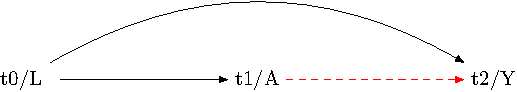
\includegraphics[width=0.8\textwidth,height=\textheight]{causal-dags_files/figure-pdf/fig-dag-common-cause-1.pdf}

}

\caption{\label{fig-dag-common-cause}Counfounding by a common cause. The
dashed red arrow indicates bias arising from the open backdoor path from
A to Y.}

\end{figure}

\hypertarget{advice-attend-to-the-temporal-order-of-all-measured-variables}{%
\subsubsection{Advice: attend to the temporal order of all measured
variables}\label{advice-attend-to-the-temporal-order-of-all-measured-variables}}

Addressing confounding by a common cause involves its adjustment. This
adjustment effectively closes the backdoor path from the exposure to the
outcome. Common adjustment methods include regression, matching, inverse
probability of treatment weighting, and G-methods (covered in
(\protect\hyperlink{ref-hernuxe1n2023a}{M. A. Hernán and Robins 2023b}).
Figure~\ref{fig-dag-common-cause-solution} clarifies that any confounder
that is a common cause of both \(A\) and \(Y\) must precede \(A\) (and
hence \(Y\)), since effects follow their causes chronologically.

By time-indexing the nodes on the graph, we see that \textbf{control of
confounding generally necessitates time-series data.}

\begin{figure}

{\centering 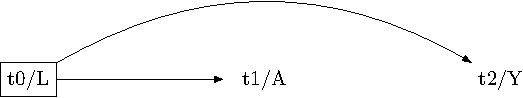
\includegraphics[width=0.8\textwidth,height=\textheight]{causal-dags_files/figure-pdf/fig-dag-common-cause-solution-1.pdf}

}

\caption{\label{fig-dag-common-cause-solution}Solution: adjust for
pre-exposure confounder.}

\end{figure}

\hypertarget{confounding-by-collider-stratification-conditioning-on-a-common-effect}{%
\subsubsection{2. Confounding by collider stratification (conditioning
on a common
effect)}\label{confounding-by-collider-stratification-conditioning-on-a-common-effect}}

Conditioning on a common effect occurs when a variable \(L\) is affected
by the treatment \(A\) and an outcome \(Y\).

Suppose \(A\) and \(Y\) are initially independent, such that
\(A \coprod Y(a)\). Conditioning on the joint effect \(L\) opens a
backdoor path between \(A\) and \(Y\), potentially inducing a non-causal
association. This occurs because \(L\) can provide information about
both \(A\) and \(Y\). Here is an example:

Let \(A\) denote the level of belief in Big Gods (with higher values
indicating stronger belief), \(Y\) denote social complexity, and \(L\)
denote economic trade. Suppose that belief in Big Gods and social
complexity are not causally linked. However, beliefs in Big Gods and
social complexity influence levels of economic trade. Suppose we were to
condition on economic trade without attending to temporal order. In that
case, we might find a statistical association between belief in Big Gods
and social complexity without a causal association.

To clarify, denote the observed associations as follows:

\begin{itemize}
\tightlist
\item
  \(P(A)\): Distribution of beliefs in Big Gods
\item
  \(P(Y)\): Distribution of social complexity
\item
  \(P(L)\): Distribution of economic trade
\end{itemize}

Without conditioning on \(L\), if \(A\) and \(Y\) are independent, we
have:

\[P(A, Y) = P(A)P(Y)\]

However, if we condition on \(L\) (which is a common effect of both
\(A\) and \(Y\)), we have:

\[P(A, Y | L) \neq P(A | L)P(Y | L)\]

Once conditioned on, the common effect \(L\) creates an association
between \(A\) and \(Y\) that is not causal. This association in the data
can mislead us into believing there is a direct link between beliefs in
Big Gods and social complexity, even without such a link. If we only
observed \(A\), \(Y\), and \(L\) in cross-sectional data, we might
erroneously conclude \(A \to Y\).\footnote{When \(A\) and \(Y\) are
  independent, the joint probability of \(A\) and \(Y\) is equal to the
  product of their individual probabilities: \(P(A, Y) = P(A)P(Y)\).
  However, when we condition on \(L\), the joint probability of \(A\)
  and \(Y\) given \(L\) is not necessarily equal to the product of the
  individual probabilities of \(A\) and \(Y\) given \(L\), hence the
  inequality \(P(A, Y | L) \neq P(A | L)P(Y | L)\).}

\begin{figure}

{\centering 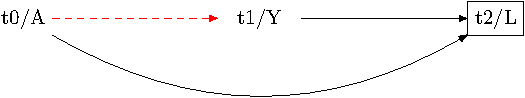
\includegraphics[width=0.8\textwidth,height=\textheight]{causal-dags_files/figure-pdf/fig-dag-common-effect-1.pdf}

}

\caption{\label{fig-dag-common-effect}Confounding by conditioning on a
collider. The dashed red arrow indicates bias from the open backdoor
path from A to Y.}

\end{figure}

\hypertarget{advice-attend-to-the-temporal-order-of-all-measured-variables-1}{%
\subsubsection{Advice: attend to the temporal order of all measured
variables}\label{advice-attend-to-the-temporal-order-of-all-measured-variables-1}}

To address the problem of conditioning on a common effect, we should
generally ensure that all confounders \(L\) that are common causes of
the exposure \(A\) and the outcome \(Y\) are measured before \(A\) has
occurred, and \(A\) is measured before \(Y\) has occurred. If such
temporal order is preserved, \(L\) cannot be an effect of \(A\), and
thus neither of \(Y\).\footnote{This rule is not absolute. As indicated
  in Figure~\ref{fig-dag-descendent-solution}, it may be helpful in
  certain circumstances to condition on a confounder that occurs after
  the outcome has occurred.} In the case of the example just described,
we require time-series data with accurate measurements. We also require
a sufficiently large sample of cultures before introducing certain
religious beliefs. Moreover, the cultures would need to be independent
of each other.\footnote{The independence of cultural units was at the
  centre of the study of comparative urban archaeology from the late
  19th (\protect\hyperlink{ref-decoulanges1903}{De Coulanges 1903})
  through the late 20th century
  (\protect\hyperlink{ref-wheatley1971}{Wheatley 1971}). Despite
  attention to this problem in recent work (e.g.
  (\protect\hyperlink{ref-watts2016}{Watts et al. 2016})), there is
  arguably a greater head-room for understanding the need for
  conditional independence of cultures in recent cultural evolutionary
  studies. Again, attending to temporal order of events is essential.}

\begin{figure}

{\centering 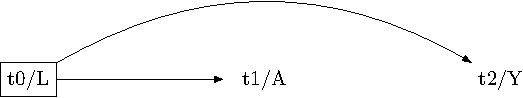
\includegraphics[width=0.8\textwidth,height=\textheight]{causal-dags_files/figure-pdf/fig-dag-common-effect-solution-1.pdf}

}

\caption{\label{fig-dag-common-effect-solution}Solution: time idexing of
confounders helps to avoid collider bias and maintain d-separation.}

\end{figure}

\hypertarget{m-bias-conditioning-on-a-collider-that-occurs-before-the-exposure-may-introduce-bias}{%
\subsubsection{M-bias: conditioning on a collider that occurs before the
exposure may introduce
bias}\label{m-bias-conditioning-on-a-collider-that-occurs-before-the-exposure-may-introduce-bias}}

Typically, indicators for confounders should be included only if they
are known to be measured before their exposures ( exceptions described
below).

However, researchers should also be cautious about over-conditioning on
pre-exposure variables that are not associated with both the exposure
and confounder, as doing so can induce confounding. As shown in
Figure~\ref{fig-m-bias}, collider stratification may arise even if \(L\)
occurs before \(A\). This happens when \(L\) does not affect \(A\) or
\(Y\), but may be the descendent of an unmeasured variable that affects
\(A\) and another unmeasured variable that also affects \(Y\).
Conditioning on \(L\) in this scenario evokes ``M-bias.'' If \(L\) is
not a common cause of \(A\) and \(Y\), or the effect of a shared common
cause, \(L\) should not be included in a causal model.
Figure~\ref{fig-m-bias} presents a case in which \(A \coprod Y(a)\) but
\(A \cancel{\coprod} Y(a)| L\). M-bias is another example of collider
stratification bias (see: (\protect\hyperlink{ref-cole2010}{Stephen R.
Cole et al. 2010})).

\begin{figure}

{\centering 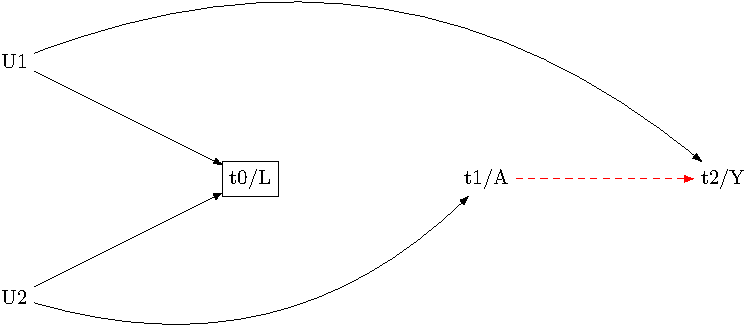
\includegraphics[width=0.8\textwidth,height=\textheight]{causal-dags_files/figure-pdf/fig-m-bias-1.pdf}

}

\caption{\label{fig-m-bias}M-bias: confounding control by including
previous outcome measures. The dashed red arrow indicates bias from the
open backdoor path from A to Y by conditioning on pre-exposure variable
L. The solution: do not condition on L.}

\end{figure}

\hypertarget{advice-adopt-the-modified-disjunctive-cause-criterion-for-confounding-control}{%
\subsubsection{Advice: adopt the modified disjunctive cause criterion
for confounding
control}\label{advice-adopt-the-modified-disjunctive-cause-criterion-for-confounding-control}}

Again, the modified disjunctive cause criterion will satisfy the
backdoor criterion in all cases and reduce bias where this criterion
cannot be fully satisfied. Again:

\begin{enumerate}
\def\labelenumi{\alph{enumi}.}
\tightlist
\item
  Control for any variable that causes the exposure, the outcome, or
  both.
\item
  Control for any proxy for an unmeasured variable that is a shared
  cause of both exposure and outcome.
\item
  Define an instrumental variable as a variable associated with the
  exposure but does not influence the outcome independently, except
  through the exposure. Exclude any instrumental variable that is not a
  proxy for an unmeasured confounder from the confounder set (see: Tyler
  J. VanderWeele, Mathur, and Chen
  (\protect\hyperlink{ref-vanderweele2020}{2020}) page 441,
  (\protect\hyperlink{ref-vanderweele2019}{Tyler J. VanderWeele 2019}))
\end{enumerate}

Of course, the difficulty is in determining which variables belong to
the desired set! Specialist knowledge can facilitate this task but
cannot generally be ascertained from the data.

\hypertarget{mediator-bias}{%
\subsubsection{3. Mediator bias}\label{mediator-bias}}

Conditioning on a mediator -- a variable that lies along the causal
pathway between the treatment and the outcome -- can distort the total
effect of the treatment on the outcome and potentially introduce bias.
To illustrate this, consider ``beliefs in Big Gods'' as the treatment
(\(A\)), ``social complexity'' as the outcome (\(Y\)), and ``economic
trade'' as the mediator (\(L\)).

In this scenario, the belief in Big Gods (\(A\)) has a direct impact on
economic trade (\(L\)), which subsequently influences social complexity
(\(Y\)). If we condition on economic trade (\(L\)), we could bias our
estimates of the overall effect of beliefs in Big Gods (\(A\)) on social
complexity (\(Y\)). This bias happens because conditioning on \(L\) can
downplay the direct effect of \(A\) on \(Y\), as it blocks the indirect
path through \(L\). This problem, known as mediator bias, is illustrated
in Figure~\ref{fig-dag-mediator}.

We might think that conditioning on a mediator does not introduce bias
under a null hypothesis (\(A\) does not cause \(Y\)), however, this is
not the case. Consider a situation where \(L\) is a common effect of the
exposure \(A\) and an unmeasured variable \(U\) linked to the outcome
\(Y\). In this scenario, including \(L\) may amplify the association
between \(A\) and \(Y\), even if \(A\) is not associated with \(Y\) and
\(U\) does not cause \(A\). This scenario is represented in
Figure~\ref{fig-dag-descendent}.

So, unless one is explicitly investigating mediation analysis, it is
usually not advisable to condition on a post-treatment variable. Paying
attention to chronology in the graph is crucial here: if we cannot
ensure that \(L\) is measured before \(A\) and \(A\) may affect \(L\),
including \(L\) in our model could result in mediator bias. This
scenario is presented in Figure~\ref{fig-dag-descendent}.

\begin{figure}

{\centering 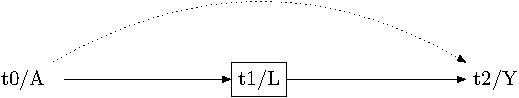
\includegraphics[width=0.8\textwidth,height=\textheight]{causal-dags_files/figure-pdf/fig-dag-mediator-1.pdf}

}

\caption{\label{fig-dag-mediator}Confounding by conditioning on a
mediator. The dashed black arrow indicates bias arising from partially
blocking the path between A and Y.}

\end{figure}

\hypertarget{advice-attend-to-the-temporal-order-of-all-measured-variables-2}{%
\subsubsection{Advice: attend to the temporal order of all measured
variables}\label{advice-attend-to-the-temporal-order-of-all-measured-variables-2}}

To mitigate the issue of mediator bias, particularly when focusing on
total effects, we should generally avoid conditioning on a mediator. We
avoid this problem by ensuring that \(L\) occurs before the treatment
\(A\) and the outcome \(Y\) (Note: a counter-example is presented in
Figure~\ref{fig-dag-descendent-solution-2}). Again, we discover the
importance of explicitly stating the temporal ordering of our
variables.\footnote{Note that if \(L\) were associated with \(Y\) and
  could not be caused by \(A\), conditioning on \(L\) would typically
  enhance the precision of the causal effect estimate of \(A \to Y\).
  This precision enhancement holds even if \(L\) occurs after \(A\).
  However, the onus is on the researcher to show that the post-treatment
  factor cannot be a consequence of the exposure.}

\begin{figure}

{\centering 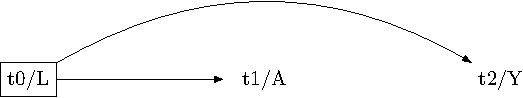
\includegraphics[width=0.8\textwidth,height=\textheight]{causal-dags_files/figure-pdf/fig-dag-mediator-solution-1.pdf}

}

\caption{\label{fig-dag-mediator-solution}Unless certain the exposure
cannot affect the confounder, ensure confounders are measured prior to
the exposure.}

\end{figure}

\hypertarget{conditioning-on-a-descendant}{%
\subsubsection{4. Conditioning on a
descendant}\label{conditioning-on-a-descendant}}

Say \(L\) is a cause of \(L^\prime\). According to Markov factorisation,
if we condition on \(L\), we partially condition on \(L^\prime\).

Consider how conditioning might imperil causal estimation. Suppose there
is a confounder \(L^\prime\) that is caused by an unobserved variable
\(U\), and is affected by the treatment \(A\). Suppose further that
\(U\) causes the outcome \(Y\). In this scenario, as described in
Figure~\ref{fig-dag-descendent}, conditioning on \(L^\prime\), which is
a descendant of \(A\) and \(U\), can lead to a spurious association
between \(A\) and \(Y\) through the path \(A \to L^\prime \to U \to Y\).

\begin{figure}

{\centering 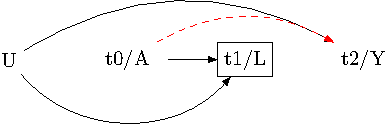
\includegraphics[width=0.8\textwidth,height=\textheight]{causal-dags_files/figure-pdf/fig-dag-descendent-1.pdf}

}

\caption{\label{fig-dag-descendent}Confounding by descent: the red
dashed arrow illustrates the introduction of bias from the opening of a
backdoor path between the exposure (A) and the outcome (Y) when
conditioning on a descendant of a confounder.}

\end{figure}

Again, the advice is clear: we should measure the (\(L^\prime\)) before
the exposure (\(A\)). This solution is presented in
Figure~\ref{fig-dag-descendent-solution}.

\begin{figure}

{\centering 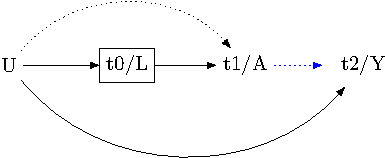
\includegraphics[width=0.8\textwidth,height=\textheight]{causal-dags_files/figure-pdf/fig-dag-descendent-solution-1.pdf}

}

\caption{\label{fig-dag-descendent-solution}Solution: again, ensure
temporal ordering for all measured variables.}

\end{figure}

Next consider how we may use a post-treatment descendent to reduce bias.
Suppose an unmeasured confounder \(U\) affects \(A\), \(Y\), and
\(L^\prime\) as presented in, then adjusting for \(L^\prime\) may help
to reduce confounding caused by \(U\). This scenario is presented in
Figure~\ref{fig-dag-descendent-solution-2}. If we deploy the modified
disjunctive cause criterion for confounding control, we would ``include
as a covariate any proxy for an unmeasured variable that is a common
cause of both the exposure and the outcome''
(\protect\hyperlink{ref-vanderweele2019}{Tyler J. VanderWeele 2019}). We
discover that although \(L^\prime\) may occur \emph{after} the exposure,
and indeed occur \emph{after} the outcome, we may condition on it to
reduce confounding because it is a proxy for an unmeasured common cause
of the exposure and the confounder. This example shows that employing a
rule that requires us to condition only on pre-exposure (and indeed
pre-outcome) variables would be hasty.

\begin{figure}

{\centering 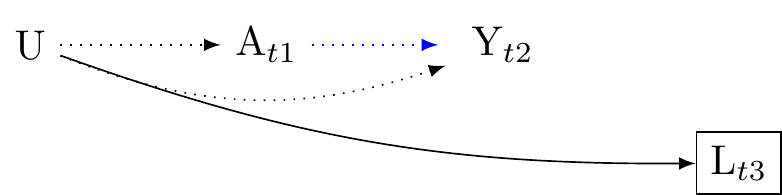
\includegraphics[width=0.8\textwidth,height=\textheight]{causal-dags_files/figure-pdf/fig-dag-descendent-solution-2-1.pdf}

}

\caption{\label{fig-dag-descendent-solution-2}Solution: conditioning on
a confounder that occurs after the exposure and the outcome may address
a problem of unmeasured confounding if the confounder is a descendent of
a prior common cause of the exposure and outcome. The dotted paths
denote that the effect of U on A and Y is partially adjusted by
conditioning on L', even though L' occurs after the outcome. The dotted
blue represents suppressing bias. For example, a genetic factor that
affects the exposure and the outcome early in life might be measured by
an indicator late that is expressed (and may be measured) later in life.
Adjusting for such an indicator would constitute an example of
post-outcome confounding control.}

\end{figure}

\hypertarget{case-1-causal-interaction-do-not-attempt-to-draw-non-linear-relationships-such-as-interactions}{%
\subsubsection{Case 1: Causal Interaction: do not attempt to draw
non-linear relationships such as
interactions}\label{case-1-causal-interaction-do-not-attempt-to-draw-non-linear-relationships-such-as-interactions}}

Interactions may be of great scientific importance. How shall we depict
interactions on a graph? It is crucial to remember the primary function
of causal diagrams is to investigate confounding. Causal diagrams are
not designed to capture all facets of a phenomenon under investigation.
We should not attempt any unique visual trick to show additive and
multiplicative interaction. Including the relevant notes and paths
necessary to evaluate sources of bias is sufficient.

Some misunderstandings can arise regarding the role and function of
causal diagrams. These often stem from a more profound confusion about
the concept of interaction itself. Given this, it is worth clarifying
the notion of interaction within a counterfactual causal framework.
Again, evaluating evidence for interaction is often essential to much
scientific research. However, we must distinguish between concepts of
causal interaction and concepts of causal effect modification.

\hypertarget{depicting-causal-interaction-in-two-independent-exposures}{%
\paragraph{\texorpdfstring{\textbf{Depicting causal interaction in two
independent
exposures}}{Depicting causal interaction in two independent exposures}}\label{depicting-causal-interaction-in-two-independent-exposures}}

Causal interaction refers to the combined or separate (or non-existent)
effect of two exposures. Evidence for interaction on a given scale is
present when the effect of one exposure on an outcome hinges on another
exposure's level. For instance, the impact of beliefs in Big Gods
(exposure A) on social complexity (outcome Y) might be contingent on a
culture's monumental architecture (exposure B), which could also
influence social complexity. Evidence of causal interaction on the
difference scale would be present if:

\[\bigg(\underbrace{E[Y(1,1)]}_{\text{joint exposure}} - \underbrace{E[Y(0,0)]}_{\text{neither exposed}}\bigg) - \bigg[ \bigg(\underbrace{E[Y(1,0)]}_{\text{only A exposed}} - \underbrace{E[Y(0,0)]}_{\text{neither exposed}}\bigg) + \bigg(\underbrace{E[Y(0,1)]}_{\text{only B exposed}} - \underbrace{E[Y(0,0)]}_{\text{neither exposed}} \bigg)\bigg] \neq 0 \]

This equation simplifies to

\[ \underbrace{E[Y(1,1)]}_{\text{joint exposure}} - \underbrace{E[Y(1,0)]}_{\text{only A exposed}} - \underbrace{E[Y(0,1)]}_{\text{only B exposed}} + \underbrace{E[Y(0,0)]}_{\text{neither exposed}} \neq 0 \]

If the above equation were to hold, the effect of exposure \(A\) on the
outcome \(Y\) would differ across levels of \(B\) or vice versa. Such a
difference would provide evidence for interaction.

If the value is positive, we say there is evidence for an additive
effect. If the value is less than zero, we say there is evidence for a
sub-additive effect. If the value is virtually zero, there is no
reliable evidence for interaction.\footnote{Note that causal effects of
  interactions often differ when measured on the ratio scale. This
  discrepency can have significant policy implications, see:
  (\protect\hyperlink{ref-vanderweele2014}{Tyler J. VanderWeele and Knol
  2014}). Although beyond the scope of this article, when evaluating
  evidence for causality we must clarify the measure of effect in which
  we are interested (\protect\hyperlink{ref-hernuxe1n2004}{Miguel A.
  Hernán, Hernández-Díaz, and Robins 2004};
  \protect\hyperlink{ref-tripepi2007}{Tripepi et al. 2007}).}

Remember that causal diagrams are non-parametric. They do not directly
represent interactions. They are tools for addressing the identification
problem. Although a causal diagram can indicate an interaction's
presence by displaying two exposures jointly influencing an outcome, as
in Figure~\ref{fig-dag-interaction}, it does not directly represent the
interaction's nature or scale.

\begin{figure}

{\centering 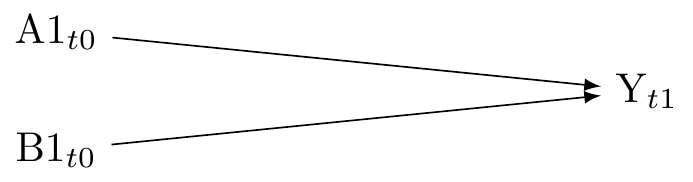
\includegraphics[width=0.6\textwidth,height=\textheight]{causal-dags_files/figure-pdf/fig-dag-interaction-1.pdf}

}

\caption{\label{fig-dag-interaction}Causal interaction: if two exposures
are causally independent of each other, we may wish to estimate their
individual and joint effects on Y, where the counterfactual outcome is
Y(a,b) and there is evidence for additive or subadditive interaction if
E{[}Y(1,1) - Y(0,1) - Y(1,0) + Y(0,0){]} ≠ 0. If we cannot conceptualise
B as a variable upon which intervention can occur, then the interaction
is better conceived as effect modification (see next figure). Important:
do not attempt to draw a path into another path.}

\end{figure}

\hypertarget{understanding-effect-modification}{%
\paragraph{\texorpdfstring{\textbf{Understanding effect
modification}}{Understanding effect modification}}\label{understanding-effect-modification}}

With the analysis of effect modification, we aim to understand how an
exposure's effect varies, if at all, across levels of another variable,
an effect modifier.

Suppose we are investigating how the impact of belief in Big Gods on
social complexity varies across early urban civilisations in ancient
China and South America. Here, geography (China versus South America) is
an ``effect modifier.'' Importantly, we are not treating the effect
modifier as an intervention. Rather, we wish to investigate whether
geography is a parameter that may alter the exposure's effect on an
outcome.

For clarity, consider comparing two exposure levels, represented as
\(A = a\) and \(A= a^*\). Further, assume that \(G\) represents two
levels of effect-modification, represented as \(g\) and \(g'\).

Then, the expected outcome when exposure is at level \(A=a\) among
individuals in group \(G=g\) is expressed

\[\hat{E}[Y(a)|G=g]\]

The expected outcome when exposure is at level \(A=a^*\) among
individuals in group \(G=g\) is expressed

\[\hat{E}[Y(a^*)|G=g]\]

The causal effect of shifting the exposure level from \(a^*\) to \(a\)
in group \(g\) is expressed

\[\hat{\delta}_g = \hat{E}[Y(a)|G=g] - \hat{E}[Y(a^*)|G=g]\]

Likewise, the causal effect of changing the exposure from \(a^*\) to
\(a\) in group \(g'\) is expressed

\[\hat{\delta}_{g'} = \hat{E}[Y(a)|G=g'] - \hat{E}[Y(a^*)|G=g']\]

We compare the causal effect on the difference scale in these two groups
by computing

\[\hat{\gamma} = \hat{\delta}_g - \hat{\delta}_{g'}\]

The value of \(\hat{\gamma}\) quantifies how the effect of shifting the
exposure from \(a^*\) to \(a\) differs between groups \(g\) and \(g'\).

If \(\hat{\gamma}\neq 0\), then there is evidence for effect
modification. We may infer the exposure's effect varies by geography.

Again, remember that causal diagrams are non-parametric. Do not draw an
intersecting path or attempt other visualisations to represent effect
modification. Instead, draw two edges into the exposure. This is
depicted in Figure~\ref{fig-dag-effect-modfication}. Always remember
that the primary goal of creating a causal diagram is to evaluate
confounding.\footnote{For important distinctions within effect
  modification, see (\protect\hyperlink{ref-vanderweele2007}{Tyler J.
  VanderWeele and Robins 2007}).}

\begin{figure}

{\centering 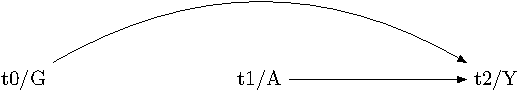
\includegraphics[width=0.8\textwidth,height=\textheight]{causal-dags_files/figure-pdf/fig-dag-effect-modfication-1.pdf}

}

\caption{\label{fig-dag-effect-modfication}A simple graph for
effect-modification.}

\end{figure}

\hypertarget{case-2-causal-mediation-causal-diagrams-show-the-inadequacy-of-standard-approaches}{%
\subsubsection{Case 2: Causal Mediation: causal diagrams show the
inadequacy of standard
approaches}\label{case-2-causal-mediation-causal-diagrams-show-the-inadequacy-of-standard-approaches}}

The conditions necessary for causal mediation are stringent. I present
these conditions in the chronologically ordered causal diagram shown in
Figure~\ref{fig-dag-mediation-assumptions}. We will again consider
whether cultural beliefs in Big Gods affect social complexity. Let us
also ask whether this affect is mediated by political authority. The
assumptions required for asking causal mediation questions are as
follows

\begin{enumerate}
\def\labelenumi{\arabic{enumi}.}
\tightlist
\item
  \textbf{No unmeasured exposure-outcome confounders given} \(L\)
\end{enumerate}

This prerequisite is expressed as \(Y(a,m) \coprod A | L1\). Upon
controlling for the covariate set \(L1\), we must ensure that no
additional unmeasured confounders affect both the cultural beliefs in
Big Gods \(A\) and the social complexity \(Y\). For example, suppose our
study involves the effect of cultural beliefs in Big Gods (exposure) on
social complexity (outcome), and geographic location and historical
context define the covariates in \(L1\). In that case, we must assume
that accounting for \(L1\) ensures d-separation of \(A\) and \(Y\). The
relevant confounding path is depicted in brown in
Figure~\ref{fig-dag-mediation-assumptions}.

\begin{enumerate}
\def\labelenumi{\arabic{enumi}.}
\setcounter{enumi}{1}
\tightlist
\item
  \textbf{No unmeasured mediator-outcome confounders given} \(L\)
\end{enumerate}

This condition is expressed as \(Y(a,m) \coprod M | L2\). After
controlling for the covariate set \(L2\), we must ensure that no other
unmeasured confounders affect the political authority \(M\) and social
complexity \(Y\). For instance, if trade networks impact political
authority and social complexity, we must account for trade networks to
obstruct the unblocked path linking our mediator and outcome. Further,
we must assume the absence of any other confounders for the
mediator-outcome path. This confounding path is represented in blue in
Figure~\ref{fig-dag-mediation-assumptions}.

\begin{enumerate}
\def\labelenumi{\arabic{enumi}.}
\setcounter{enumi}{2}
\tightlist
\item
  \textbf{No unmeasured exposure-mediator confounders given} \(L\)
\end{enumerate}

This requirement is expressed as \(M(a) \coprod A | L3\). Upon
controlling for the covariate set \(L3\), we must ensure that no
additional unmeasured confounders affect both the cultural beliefs in
Big Gods \(A\) and political authority \(M\). For example, the
capability to construct large ritual theatres may influence the belief
in Big Gods and the level of political authority. If we have indicators
for this technology measured prior to the emergence of Big Gods (these
indicators being \(L3\)), we must assume that accounting for \(L3\)
closes the backdoor path between the exposure and the mediator. This
confounding path is shown in green in
Figure~\ref{fig-dag-mediation-assumptions}.

\begin{enumerate}
\def\labelenumi{\arabic{enumi}.}
\setcounter{enumi}{3}
\tightlist
\item
  \textbf{No mediator-outcome confounder affected by the exposure (no
  red arrow)}
\end{enumerate}

This requirement is expressed as \(Y(a,m) \coprod M(a^*) | L\). We must
ensure that no variables confounding the relationship between political
authority and social complexity in \(L2\) are themselves influenced by
the cultural beliefs in Big Gods (\(A\)). For instance, when studying
the effect of cultural beliefs in Big Gods (\(A\), the exposure) on
social complexity (\(Y\), the outcome) as mediated by political
authority (mediator), there can be no factors, such as trade networks
(\(L2\)), that influence both political authority and social complexity
and are affected by the belief in Big Gods. This confounding path is
shown in red in Figure~\ref{fig-dag-mediation-assumptions}. \textbf{Note
that the assumption of no exposure-induced confounding in the
mediator-outcome relationship poses a significant challenge.} If the
exposure influences a confounder of the mediator and outcome, we face a
dilemma. Without accounting for this confounder, the backdoor path
between the mediator and the outcome remains open. By accounting for it,
however, we partially obstruct the path between the exposure and the
mediator, leading to bias. Consequently, observed data cannot identify
the natural direct and indirect effects.

Notice again that the requirements for counterfactual data science are
more strict than for descriptive or predictive data science.

Nonetheless, we can set the mediator to certain levels and explore
controlled direct and indirect effects, which may be relevant to science
and policy. For instance, if we were to fix political authority at a
specific level, we could ask, what would be Big Gods' direct and
indirect causal effects on social complexity? Other approaches involve
sampling from the observed distributions to obtain probabilistic
identification (see: (\protect\hyperlink{ref-shi2021}{Shi et al. 2021})
). Answering such questions requires G-methods
(\protect\hyperlink{ref-hernuxe1n2023a}{M. A. Hernán and Robins
2023b})).

We have now considered how chronologically ordered causal diagrams
elucidate the conditions necessary for causal mediation
analysis.\footnote{An excellent resource both for understanding causal
  interaction and causal mediation is
  (\protect\hyperlink{ref-vanderweele2015}{T. VanderWeele 2015b}).}

\begin{figure}

{\centering \includegraphics[width=0.8\textwidth,height=\textheight]{causal-dags_files/figure-pdf/fig-dag-mediation-assumptions-1.pdf}

}

\caption{\label{fig-dag-mediation-assumptions}Assumptions for mediation
analysis. The brown edges denote the path for common causes of the
exposure and coutcome. To block this path we must condition on L1. The
green edges denote the path for common causes of the exposure and
mediator. To block this path we must condition on L3. The blue edges
denote the path for common causes of the mediator and outcome. To block
this path we must condition on L2. The red path denotes the effect of
the exposure on the confounder of the mediator and outcome. If any such
path exists then we cannot obtain natural direct and indirect effects.
Conditioning on L2 is necessary to prevent mediator outcome confounding
but doing so blocks the effect of the exposure on the mediator.}

\end{figure}

\hypertarget{case-3-confounder-treatment-feedback-longitudinal-growth-is-not-causation}{%
\subsubsection{Case 3: Confounder-Treatment Feedback: Longitudinal
``growth'' is not
causation}\label{case-3-confounder-treatment-feedback-longitudinal-growth-is-not-causation}}

In our discussion of causal mediation, we consider how the effects of
two sequential exposures may combine to affect an outcome. We can
broaden this interest to consider the causal effects of multiple
sequential exposures. In such scenarios, causal diagrams arranged
chronologically can aid in clarifying the challenges and opportunities.

For example, consider temporally fixed multiple exposures. The
counterfactual outcomes may be denoted \(Y(a_{t1} ,a_{t2})\). There are
four counterfactual outcomes corresponding to the four fixed ``treatment
regimes'':

\begin{enumerate}
\def\labelenumi{\arabic{enumi}.}
\item
  \textbf{Always treat (Y(1,1))}
\item
  \textbf{Never treat (Y(0,0))}
\item
  \textbf{Treat once first (Y(1,0))}
\item
  \textbf{Treat once second (Y(0,1))}
\end{enumerate}

\hypertarget{tbl-regimes}{}
\begin{longtable}[]{@{}
  >{\raggedright\arraybackslash}p{(\columnwidth - 4\tabcolsep) * \real{0.1351}}
  >{\raggedright\arraybackslash}p{(\columnwidth - 4\tabcolsep) * \real{0.5405}}
  >{\raggedright\arraybackslash}p{(\columnwidth - 4\tabcolsep) * \real{0.3243}}@{}}
\caption{\label{tbl-regimes}Table describes four fixed treatment regimes
and six causal contrasts in time series data where the exposure may
vary.}\tabularnewline
\toprule\noalign{}
\begin{minipage}[b]{\linewidth}\raggedright
Type
\end{minipage} & \begin{minipage}[b]{\linewidth}\raggedright
Description
\end{minipage} & \begin{minipage}[b]{\linewidth}\raggedright
Counterfactual Outcome
\end{minipage} \\
\midrule\noalign{}
\endfirsthead
\toprule\noalign{}
\begin{minipage}[b]{\linewidth}\raggedright
Type
\end{minipage} & \begin{minipage}[b]{\linewidth}\raggedright
Description
\end{minipage} & \begin{minipage}[b]{\linewidth}\raggedright
Counterfactual Outcome
\end{minipage} \\
\midrule\noalign{}
\endhead
\bottomrule\noalign{}
\endlastfoot
Regime & Always treat & Y(1,1) \\
Regime & Never treat & Y(0,0) \\
Regime & Treat once first & Y(1,0) \\
Regime & Treat once second & Y(0,1) \\
Contrast & Always treat vs.~Never treat & E{[}Y(1,1) - Y(0,0){]} \\
Contrast & Always treat vs.~Treat once first & E{[}Y(1,1) - Y(1,0){]} \\
Contrast & Always treat vs.~Treat once second & E{[}Y(1,1) -
Y(0,1){]} \\
Contrast & Never treat vs.~Treat once first & E{[}Y(0,0) - Y(1,0){]} \\
Contrast & Never treat vs.~Treat once second & E{[}Y(0,0) - Y(0,1){]} \\
Contrast & Treat once first vs.~Treat once second & E{[}Y(1,0) -
Y(0,1){]} \\
\end{longtable}

There are six causal contrasts that we might compute for the four fixed
regimes, presented in Table~\ref{tbl-regimes}.\footnote{We compute the
  number of possible combinations of contrasts by
  \(C(n, r) = \frac{n!}{(n-r)! \cdot r!}\)}

Not that treatment assignments might be sensibly approached as a
function of the previous outcome. For example, we might \textbf{treat
once first} and then decide whether to treat again depending on the
outcome of the initial treatment. This aspect is known as ``time-varying
treatment regimes.''

It is important to remember that to estimate the ``effect'' of a
time-varying treatment regime, we must compare the counterfactual
quantities of interest. Just as mediation introduces the possibility of
time-varying confounding (condition 4, where the exposure affects the
confounders of the mediator/outcome path), so too do all sequential
time-varying treatments. Unlike traditional causal mediation analysis,
however, we might consider the sequence of treatment regimes
indefinitely long.

Chronologically organised causal diagrams are useful for highlighting
problems with traditional multi-level regression analysis and structural
equation modelling.

For example, we might be interested in whether belief in Big Gods
affects social complexity. Consider estimating a fixed treatment regime
first. Suppose we have a well-defined concept of Big Gods and social
complexity as well as excellent measurements for both over time. In that
case, we might want to assess the effects of beliefs in Big Gods on
social complexity, say, two centuries after the beliefs were introduced.

The fixed treatment strategies are: ``always believe in Big Gods''
versus ``never believe in Big Gods'' on the level of social complexity.
Refer to Figure~\ref{fig-dag-9}. Here, \(A_{tx}\) represents the
cultural belief in Big Gods at time \(tx\), and \(Y_{tx}\) is the
outcome, social complexity, at time \(x\). Imagine that economic trade,
denoted as \(L_{tx}\), is a time-varying confounder. Suppose its effect
changes over time, which in turns affects the factors that influence
economic trade. To complete our causal diagram, we might include an
unmeasured confounder \(U\), such as oral traditions, which could
influence both the belief in Big Gods and social complexity.

Suppose we can credibly think that the level of economic trade at time
\(0\), \(L_{t0}\), influence beliefs in ``Big Gods'' at time \(1\),
\(A_{t1}\). We therefore draw an arrow from \(L_{t0}\) to \(A_{t1}\).
But we may also think the belief in ``Big Gods'', \(A_{t1}\), affects
the future level of economic trade, \(L_{t(2)}\). Thus, we must add an
arrow from \(A_{t1}\) to \(L_{t2}\). This causal diagram represents a
feedback process between the time-varying exposure \(A\) and the
time-varying confounder \(L\). Figure~\ref{fig-dag-9} shows
exposure-confounder feedback. In a real-world setting, there would be
more arrows. However, our causal diagram needs only to show the minimum
number of arrows to exhibit the problem of exposure-confounder feedback.
As a rule, we should not clutter our causal diagrams: we should only
provide the essential details to evaluate the identification problem.

What would happen if we were to condition on the time-varying confounder
\(L_{t3}\)? Two things would occur. First, we would block all the
backdoor paths between the exposure \(A_{t2}\) and the outcome. We need
to block those paths to eliminate confounding. Therefore, conditioning
on the time-varying confounding is essential. However, paths that were
previously blocked would close. For example, the path
\(A_{t1}, L_{t2}, U, Y_{t4}\), that was previously closed would be
opened because the time-varying confounder is the common effect of
\(A_{t1}\) and \(U\). Conditioning, then, opens the path
\(A_{t1}, L_{t2}, U, Y_{t4}\). Therefore we must avoid conditioning on
the time-varying confounder. It would seem then that if we were to
condition on a confounder that is affected by the prior exposure, we are
``damned if we do'' and ``dammed if we do not.''

\begin{figure}

{\centering 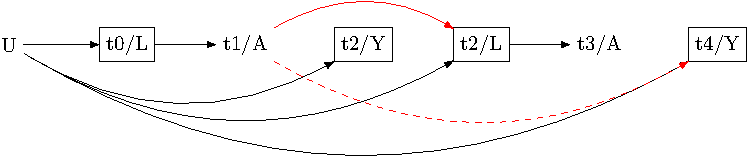
\includegraphics[width=1\textwidth,height=\textheight]{causal-dags_files/figure-pdf/fig-dag-9-1.pdf}

}

\caption{\label{fig-dag-9}Exposure confounder feedback is a problem for
time-series models. If we do not condition on L\_t2, a backdoor path is
open from A\_t3 to Y\_t4. However, if conditioning on L\_t2 introduces
collider bias, opening a path, coloured in red, between A\_t2 and Y\_t4.
Here, we may not use conventional methods to estimate the effects of
multiple exposures. Instead, at best, we may obtain controlled effects
using G-methods. Multi-level models will not eliminate bias (!).
Currently, outside of epidemiology, G-methods are rarely used.}

\end{figure}

A similar problem arises when a time-varying exposure and time-varying
confounder share a common cause. This problem arises even without the
exposure affecting the confounder. The problem is presented in
Figure~\ref{fig-dag-time-vary-common-cause-A1-l1}.

\begin{figure}

{\centering 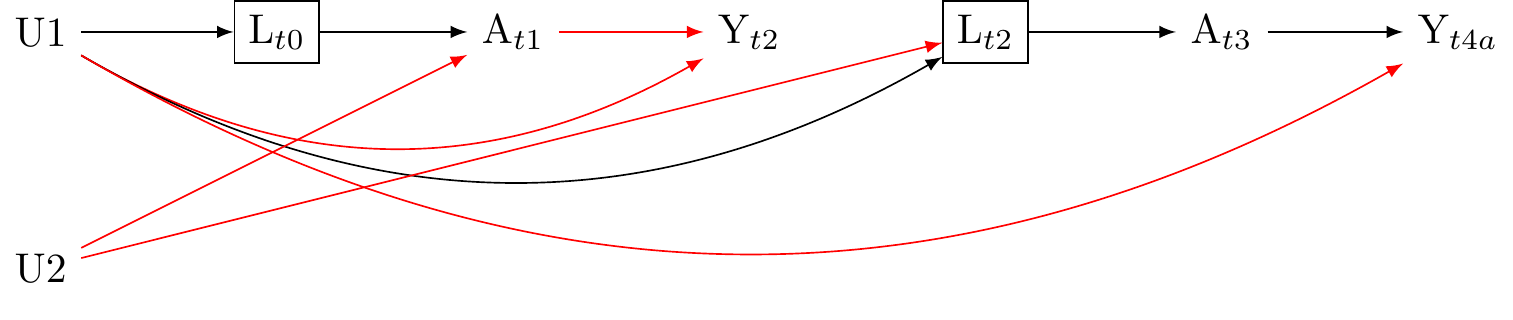
\includegraphics[width=1\textwidth,height=\textheight]{causal-dags_files/figure-pdf/fig-dag-time-vary-common-cause-A1-l1-1.pdf}

}

\caption{\label{fig-dag-time-vary-common-cause-A1-l1}Exposure confounder
feedback is a problem for time-series models. Here, the problem arises
from an unmeasured variable (U\_2) that affects both the exposure A at
time 1 and the cofounder L at time 2. The red paths show the open
backdoor path when we condition on the L at time 2. Again, we cannot
infer causal effects in such scenarios by using regression-based
methods. In this setting, to address causal questions, we require
G-methods.}

\end{figure}

Complexity grows when the exposure \(A_{t1}\) influences the outcome
\(Y_{t4}\). For instance, because \(L_{t2}\) lies on the pathway from
\(A_{t1}\) to \(Y_{t4}\), conditioning on \(L_{t2}\) partially obstructs
the connection between exposure and outcome. Such conditioning triggers
both collider stratification bias and mediator bias. However, to close
the open backdoor path between \(L_{t2}\) and \(Y_{t4}\), conditioning
on \(L_{t2}\) is necessary. Yet we have just said that we must not
condition. The broader challenge of exposure-confounder feedback is
detailed in (\protect\hyperlink{ref-hernuxe1n2023a}{M. A. Hernán and
Robins 2023b}). This issue poses a significant problem for cultural
evolutionary studies, and conventional regression-based methods ---
including multi-level models --- are incapable of solving it
(\protect\hyperlink{ref-hernuxe1n2006}{Miguel A. Hernán and Robins
2006}; \protect\hyperlink{ref-robins1999}{J. M. Robins, Greenland, and
Hu 1999}; \protect\hyperlink{ref-robins1986}{J. Robins 1986}). As
mentioned, models suited for evaluating the causal effects of time-fixed
and time-varying exposures are encompassed by ``G-methods''
(\protect\hyperlink{ref-naimi2017}{Naimi, Cole, and Kennedy 2017};
\protect\hyperlink{ref-chatton2020}{Chatton et al. 2020};
\protect\hyperlink{ref-hernuxe1n2006}{Miguel A. Hernán and Robins
2006}). Even though such methods have seen considerable development
recently in the health sciences
(\protect\hyperlink{ref-williams2021}{Williams and Díaz 2021};
\protect\hyperlink{ref-duxedaz2021}{Díaz et al. 2021};
\protect\hyperlink{ref-breskin2020}{Breskin et al. 2020}), their
adoption in cultural evolutionary research is still fledgling.
\footnote{It is worth noting that the identification of controlled
  effect estimates can benefit from graphical methods such as ``Single
  World Intervention Graphs'' (SWIGs), which depict counterfactual
  outcomes on the diagrams. Nevertheless, SWIGs, in their general form,
  are templates rather than causal diagrams. The application of SWIGS
  extends beyond this tutorial's scope. Refer to Richardson and Robins
  (\protect\hyperlink{ref-richardson2013}{2013}) for more about SWIGs.}

\hypertarget{summary-part-2}{%
\subsubsection{Summary Part 2}\label{summary-part-2}}

To consistently estimate causal effects, we must contrast the world as
it has been with the world as it might have been. For many questions in
cultural evolution, we have seen that confounder-treatment feedback
leads to intractable causal identification problems. We have also seen
that causal diagrams are helpful in clarifying these problems. Many
self-inflicted injuries, such as mediator bias and post-stratification
bias, could be avoided if confounders were measured prior to the
exposures. Chronologically ordered causal diagrams aim to make this
basis transparent.

I next turn to three-wave designs for estimating the total causal
effects. Such designs find inspiration from chronologically ordered
causal diagrams. They may be beneficial for evolutionary anthropologists
who wish to collect time-series data in the present and future to
address causal questions.

\hypertarget{part-3.-applications-of-causal-diagrams-to-the-understanding-of-data-collection-in-a-three-wave-panel-design}{%
\subsection{Part 3. Applications of Causal Diagrams to the Understanding
of Data Collection in a Three-Wave Panel
Design}\label{part-3.-applications-of-causal-diagrams-to-the-understanding-of-data-collection-in-a-three-wave-panel-design}}

In this section, we discuss how temporally ordered causal diagrams can
help illustrate the benefits of a three-wave panel design in addressing
causal queries using data.

\hypertarget{step-1.-defining-the-exposure-measure-it-at-wave-0-and-wave-1}{%
\subsubsection{Step 1. Defining the exposure: measure it at wave 0 and
wave
1}\label{step-1.-defining-the-exposure-measure-it-at-wave-0-and-wave-1}}

We start with a well-defined exposure. Unless our focus lies in causal
interaction, causal mediation, or sequential treatment plans, our task
will be to examine the total effect of a single exposure.

Consider the causal effect of attending religious services. Our primary
task is to define the exposure as a hypothetical intervention. What
interests us? Any attendance versus non-attendance? Weekly attendance
versus monthly attendance? Or is it something else? Imagining a
hypothetical experiment, even if impractical, highlights the importance
of specifying an explicit intervention
(\protect\hyperlink{ref-hernuxe1n2022}{Miguel A. Hernán, Wang, and Leaf
2022b}; \protect\hyperlink{ref-hernuxe1n2016a}{Miguel A. Hernán et al.
2016b}).

Controlling for the exposure at the baseline also has an additional
benefit: it can lower the probability of bias from unmeasured
confounders. We shall say more about this benefit after introducing the
next step.

\hypertarget{note-without-access-to-an-exposed-populationif-the-exposure-is-rare-many-observations-must-be-collected-to-estimate-causal-effects}{%
\paragraph{\texorpdfstring{\textbf{Note: without access to an exposed
population,if the exposure is rare, many observations must be collected
to estimate causal
effects}}{Note: without access to an exposed population,if the exposure is rare, many observations must be collected to estimate causal effects}}\label{note-without-access-to-an-exposed-populationif-the-exposure-is-rare-many-observations-must-be-collected-to-estimate-causal-effects}}

Assume in the non-religious population, the switch from no religious
service attendance to weekly attendance is rare, say 1 in 1,000
non-attenders per year. Acquiring an adequate sample for a ``treatment''
group while conditioning on a rich set of variables might not be
feasible without hundreds of thousands of participants. It might be more
practical to consider changes within the religious population, assuming
changes are more common within this group. However, we would then
typically estimate a causal effect that generalises to the religious
population from which the sample was drawn rather than one that
transports to the non-religious population.

\hypertarget{step-2.-define-the-outcomes-measure-them-at-wave-0-and-wave-2}{%
\subsubsection{Step 2. Define the outcome(s): measure them at wave 0 and
wave
2}\label{step-2.-define-the-outcomes-measure-them-at-wave-0-and-wave-2}}

After defining the exposure, we need to specify a well-defined outcome
or multiple outcomes. For instance, we might be interested in how
gaining or losing religious service affects the frequency of
volunteering (e.g., weekly, monthly, yearly). Vague concepts such as
``the causal effects of religious change'' do not bring understanding.
We must specify what the phenomenon we wish to study, and the timing of
its occurrence (e.g.~the + 1-year effect on weekly volunteering from a
movement of 0 to weekly or more religious service attendance.)

It is crucial to control for the outcome measured at the baseline -- the
`baseline outcome' -- to verify the correct temporal order of the
cause-effect relationship, i.e., to prevent reverse causation.

Moreover, when we also control for the exposure at the baseline, then
for an unmeasured confounder to explain away the association between the
exposure at one wave from the baseline and the outcome at two waves from
the baseline, it would need to do so independently of the baseline
effect. This scenario is depicted in Figure~\ref{fig-dag-6}. This causal
diagram makes an essential practical point: although confounding might
not be entirely eliminated (the dashed arrows symbolise the potential
for uncontrolled sources of bias), data collection and analysis can
reduce bias. Given we can rarely be sure we have controlled for
unmeasured confounding, researchers should perform sensitivity analyses
(see: (\protect\hyperlink{ref-shi2021}{Shi et al. 2021})).

Note that I use the term ``wave'' without defining a specific period.
Causes must precede effects, but the amount of time needed to assess
causality will vary depending on the phenomena of interest. In a causal
diagram, \textbf{intervals need not be drawn to scale.}

\begin{figure}

{\centering 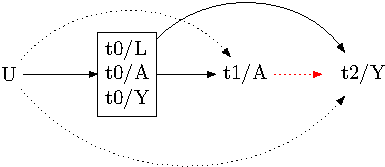
\includegraphics[width=0.8\textwidth,height=\textheight]{causal-dags_files/figure-pdf/fig-dag-6-1.pdf}

}

\caption{\label{fig-dag-6}Causal diagram adapted from Vanderweele et
al.'s three-wave panel design. The blue-dotted line indicates a
reduction in bias arising from including baseline measures for the
exposure and outcome. For an unmeasured confounder U to bias the
exposure-outcome association, it would need to do so independently of
these outcome and exposure baseline measures. The graph clarifies that
by measuring confounders before the exposure and the exposure before the
outcome, we reduce the potential for reverse causation, collider
stratification, and mediator biases.}

\end{figure}

\hypertarget{step-3.-identify-observable-common-causes-of-the-exposure-and-the-outcome}{%
\subsubsection{Step 3. Identify observable common causes of the exposure
and the
outcome}\label{step-3.-identify-observable-common-causes-of-the-exposure-and-the-outcome}}

Next, we should identify all the potential confounders that, when
adjusted for, can eliminate any non-causal association between the
exposure and outcome. We should group these confounders under standard
labels wherever they share the same functional dependencies in the
graph. In a three-wave panel design, confounders are recorded during the
baseline wave. As illustrated in Figure~\ref{fig-dag-mediator-solution},
recording confounders before the occurrence of the exposure minimises
the potential for mediation bias.

\hypertarget{step-4.-gather-data-for-proxy-variables-of-unmeasured-common-causes-at-the-baseline-wave}{%
\subsubsection{Step 4. Gather data for proxy variables of unmeasured
common causes at the baseline
wave}\label{step-4.-gather-data-for-proxy-variables-of-unmeasured-common-causes-at-the-baseline-wave}}

Recall Figure~\ref{fig-dag-descendent-solution-2}: if any unmeasured
factors influence both the exposure and outcome, but we lack direct
measurements for them, we should make efforts to include proxies for
them. Again, even if this strategy cannot eliminate all bias from
unmeasured confounding, it might reduce bias.

\hypertarget{step-5.-state-the-target-population-for-whom-the-causal-question-applies}{%
\subsubsection{Step 5. State the target population for whom the causal
question
applies}\label{step-5.-state-the-target-population-for-whom-the-causal-question-applies}}

We need to define for whom our causal inference applies. For this
purpose, it is helpful to distinguish the concepts of source population
and target population and between the concepts of generalisability and
transportability.

\begin{enumerate}
\def\labelenumi{\arabic{enumi}.}
\item
  \textbf{The source population} is the population from whom our sample
  is drawn.
\item
  \textbf{The target population} is the larger group to which we aim to
  apply our study's results. The closer the source population matches
  the target population in structural features relevant to our causal
  questions, the stronger our causal inferences about the target
  population will be.
\item
  \textbf{Generalisability}: when the causal effect estimated from a
  sample applies to the target population beyond the sample population,
  we say the causal effect estimates are generalisable. This concept is
  also known as ``external validity.''
\end{enumerate}

Let \(PATE\) denote the population average treatment effect for the
target population. Let \(ATE_{\text{source}}\) denote the average
treatment effect in the source population. Let \(W\) denote a set of
variables upon which the source and target population structurally
differ. We say that results \emph{generalise} if there is a function
such that

\[PATE =  f(ATE_{\text{source}}, W)\]

\begin{enumerate}
\def\labelenumi{\arabic{enumi}.}
\setcounter{enumi}{3}
\tightlist
\item
  \textbf{Transportability}: when causal effects estimates may
  generalise to different settings and populations from which the source
  population was sampled, we say effects are transportable. Where \(T\)
  denotes a set of variables upon which the source and the target
  population structurally differ, we say that results are transportable
  if there is a function such that
\end{enumerate}

\[ATE_{\text{target}} \approx f(ATE_{\text{source}}, T)\]

This function similarly maps the average treatment effect from the
source population to a target population. The function over \(T\) might
be more complex, as it must handle potential heterogeneity of effects
and unobserved sources of bias. To assess transportability, we generally
require information about the source and target populations and a
specialist understanding. In Section 4, we will return to the concepts
of generalisability and transportability as they pertain to sample
selection.

\hypertarget{step-6.-retention-is-a-top-priority}{%
\subsubsection{Step 6. Retention is a top
priority}\label{step-6.-retention-is-a-top-priority}}

Sample retention is a mission-critical imperative for reasons we clarify
in Part 4. Panel attrition opens novel pathways for bias. Researchers
must develop protocols for tracking individuals as they change
addresses, emails, phone numbers, and names. Moreover, developing and
implementing strategies for motivating retention across the entire
population of interest (not merely those willing to volunteer for
science) is critical for causal human science. These strategies must be
developed with specialist knowledge of the population under study and
the participation and insights of the people being studied.

\hypertarget{summary-of-part-3}{%
\subsubsection{Summary of Part 3}\label{summary-of-part-3}}

The strengths of three-wave panel designs for confounding control are
demonstrated in Figure~\ref{fig-dag-6}. This diagram, adapted from Tyler
J. VanderWeele, Mathur, and Chen
(\protect\hyperlink{ref-vanderweele2020}{2020}), highlights the
potential for residual unmeasured confounding even after incorporating
baseline measurements for both the exposure and outcome, represented by
the blue-dotted line. As such, for an unmeasured confounder \(U\) to
exert bias on the association between the exposure \(A_{t1}\) and
outcome \(Y_{t2}\), it must do so independently of the baseline
measurements of the exposure \(A_{t0}\) and outcome \(Y_{t0}\).

The diagram also clarifies the advantage of three-wave panel designs in
addressing reverse causation. This control is achieved by adjusting for
both the exposure and outcome at baseline, ensuring the temporal
sequence causality required. Moreover, the diagram underscores the
capacity of three-wave panel designs to yield estimates for the
incidence, not just the prevalence, of effects.

A further understanding gained from Figure~\ref{fig-dag-6} is related to
the potential risks associated with collider stratification and mediator
bias. As discussed in Part 2. bias may arise from conditioning on a
variable measured after treatment. We can significantly reduce such
biases by ensuring the measurement of confounders takes place before the
exposure and by ensuring that the exposure is measured before the
outcome.

Figure~\ref{fig-dag-6} emphasises these factors' crucial role in guiding
the collection of repeated measures data. Nonetheless, Tyler J.
VanderWeele, Mathur, and Chen
(\protect\hyperlink{ref-vanderweele2020}{2020})'s causal diagram does
not account for potential bias from panel attrition. In Part 4, we will
expand this graph to discuss these challenges.

\hypertarget{part-4.-applications-of-causal-diagrams-to-the-understanding-of-selection-bias}{%
\subsection{Part 4. Applications of Causal Diagrams to the Understanding
of Selection
Bias}\label{part-4.-applications-of-causal-diagrams-to-the-understanding-of-selection-bias}}

\hypertarget{introduction-to-selection-bias}{%
\subsubsection{Introduction to selection
bias}\label{introduction-to-selection-bias}}

\emph{Selection bias} may be broadly defined as the discrepancy between
the parameter of interest in a target population and the same parameter
in a subset of the population used for analysis - the source population
(\protect\hyperlink{ref-hernuxe1n2017}{M. A. Hernán 2017}). This bias
can occur if the source population differs from the target population
regarding descriptive parameters. In causal inference, our concern is
how selection bias might impact the estimation of causal effects. In
other words, how might differences between the source and target
populations influence causal contrasts on specific scales of interest
(difference, risk ratio, rate ratio, or another)? Causal diagrams help
to clarify what is at stake.

It is useful first to consider the following topology of confounding
developed by Suzuki and colleagues
(\protect\hyperlink{ref-suzuki2016}{Suzuki et al. 2016};
\protect\hyperlink{ref-suzuki2014}{Suzuki and Yamamoto 2014};
\protect\hyperlink{ref-suzuki2020}{Suzuki, Shinozaki, and Yamamoto
2020}).\footnote{This typology builds on VanderWeele's work
  (\protect\hyperlink{ref-vanderweele2012}{Tyler J. VanderWeele and
  Hernán 2012}).}

\begin{enumerate}
\def\labelenumi{\arabic{enumi}.}
\item
  \textbf{Confounding in Distribution}: if the sample exposed to each
  level of exposure is representative of the target population, we say
  there is no confounding in the distribution of the exposure's effect
  on the outcome.
\item
  \textbf{Confounding in Expectation} If the exposure assignment
  mechanism balances the confounders across each level of contrast in
  the exposure, we say there is no confounding in the expectation of the
  exposure's effect on the outcome.
\item
  \textbf{Confounding in Measure}: if a specific measure of interest
  matches the corresponding causal measure in the target population, we
  say there is no confounding in the measure of the exposure's effect on
  the outcome. As discussed previously concerning interaction, our
  inference of a causal effect can depend on the scale of the causal
  effect measure.
\item
  \textbf{Realised confounding}: if a specific exposure assignment leads
  to balance, irrespective of the exposure assignment mechanism, we say
  there is no realised confounding of the exposure's effect on the
  outcome. This concept is essential because, even in randomised
  experiments, randomisation might not eliminate chance imbalances in
  the distributions of confounders across the exposures.
\end{enumerate}

Each of these four concepts plays a role in ``confounding'' discussions,
and all are crucial when evaluating a study's scientific merit. However,
each concept highlights different issues.

Armed with these distinctions, consider
Figure~\ref{fig-selection-under-the-null}, which presents a scenario
with no (marginal) causal effect of exposure on the outcome, yet a
degree of selection into the study. We will assume randomisation
succeeded and that are no arrows into \(A\). As
Figure~\ref{fig-selection-under-the-null} shows, neither confounding in
expectation nor confounding in distribution is present. Failure to
detect an association will accurately reflect the actual state of causal
disassociation in the population. We might say that selection leads to
``confounding in distribution for confounding in expectation.'' More
simply, we might say that despite selection, the null effect in the
source population is not biased for the target population
(\protect\hyperlink{ref-hernuxe1n2004}{Miguel A. Hernán, Hernández-Díaz,
and Robins 2004}; \protect\hyperlink{ref-greenland1977}{Greenland
1977}). Note that therm ``null effect'' is a structural concept. There
are no statistical ``null effects.'' Instead there are reliable or
unreliable statistical effect estimates according to some measure of
evidence and arbitrary threshold
(\protect\hyperlink{ref-bulbulia2021}{J. Bulbulia et al. 2021}).

\begin{figure}

{\centering 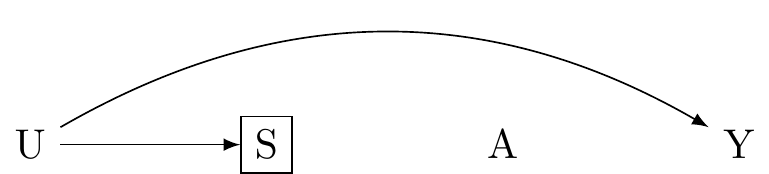
\includegraphics[width=0.6\textwidth,height=\textheight]{causal-dags_files/figure-pdf/fig-selection-under-the-null-1.pdf}

}

\caption{\label{fig-selection-under-the-null}Selection under the null.
An unmeasured variable affects the selection for the study and the
outcome. D-separation is preserved; there is no confounding in
expectation.}

\end{figure}

Figure~\ref{fig-selection-off-the-null} presents a different scenario in
which there is selection bias for the population parameter: the
association in the population of selected individuals differs from the
causal association in the target population. Hernán calls this scenario
``selection bias off the null''
(\protect\hyperlink{ref-hernuxe1n2017}{M. A. Hernán 2017}). Lu et
al.~call this scenario ``type 2 selection bias''
(\protect\hyperlink{ref-lu2022}{Lu et al. 2022}). This bias occurs
because the selection into the study occurs on an effect modifier for
the effect of the exposure on the outcome. Note that although the causal
effect of \(A\to Y\) is unbiased for the exposed and unexposed in the
source population, the effect estimate does not generalise to the
exposed and unexposed in the target population:
\(PATE \cancel{\approx} ATE_{\text{sample}}\).

\begin{figure}

{\centering 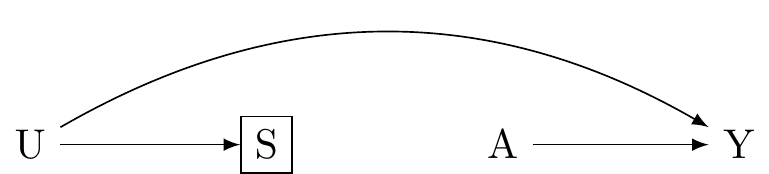
\includegraphics[width=0.6\textwidth,height=\textheight]{causal-dags_files/figure-pdf/fig-selection-off-the-null-1.pdf}

}

\caption{\label{fig-selection-off-the-null}Selection of the null: an
unmeasured variable affects selection into the study and the outcome.
Here the exposure affects the outcome. Although d-separation is
preserved, there is `confounding in distribution'.}

\end{figure}

There has been considerable technical research investigating the
conditions under which causal estimates for a target population may be
identified when the source population differs from the target population
(see: (\protect\hyperlink{ref-lu2022}{Lu et al. 2022})). There has also
been considerable technical research investigating the conditions in
which results might transport to populations that systematically differ
from the source population (see:
(\protect\hyperlink{ref-bareinboim2022}{Bareinboim, Tian, and Pearl
2022}; \protect\hyperlink{ref-pearl2022}{Pearl and Bareinboim 2022};
\protect\hyperlink{ref-deffner2022}{Deffner, Rohrer, and McElreath
2022})).To address type 2 selection bias in a three-wave pane, we must
accurately measure and adjust for a sufficient set of covariates that
affect selection \(\framebox{S}\) (\protect\hyperlink{ref-lu2022}{Lu et
al. 2022}). Moreover, when drawing causal diagrams, it is vital to
present confounding as it is assumed to exist in the target population,
not the source population (see Suzuki, Shinozaki, and Yamamoto
(\protect\hyperlink{ref-suzuki2020}{2020}), especially their examples in
the supplement.)

\hypertarget{selection-bias-in-which-both-the-exposure-and-outcome-affect-censoring}{%
\subsubsection{Selection bias in which both the exposure and outcome
affect
censoring}\label{selection-bias-in-which-both-the-exposure-and-outcome-affect-censoring}}

In panel designs, there is additionally a constant threat of selection
occurring \emph{after} enrolment into the study. We next put
chronological causal diagrams to use to make sense of this threat and
derive practical advice.

We next use causal diagrams to clarify biases arising from panel
attrition. Panel attrition can be viewed as a special case of selection
bias because the participants who continue in a longitudinal study may
differ from those who drop out in ways that generate structural biases.

Figure~\ref{fig-dag-8-5} describes a scenario in which both the exposure
and the true outcome affect panel attrition, biasing the observed
association between the exposure and the measured outcome in the
remaining sample. The problem of selection here is a problem of collider
stratification bias. We can equivalently view the problem as one of
directed measurement error, described in in
Figure~\ref{fig-dag-indep-d-effect}. Either way, restricting the
analysis to the retained sample introduces bias in the causal effect
estimate by opening a backdoor path from the exposure to the outcome. Lu
et al. (\protect\hyperlink{ref-lu2022}{2022}) call this form of bias:
``type 1 selection bias'' and distinguishes between scenarios when
causal effects that generalise are recoverable (type 1a selection bias)
and not recoverable (type 1b selection bias). In both cases, we must
develop strategies to recover target population estimates from a subset
of the source population for which causal effect estimates may be biased
\textbf{for the source population.}

\begin{figure}

{\centering 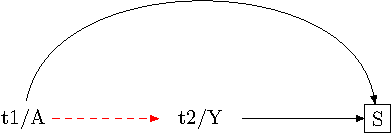
\includegraphics[width=0.8\textwidth,height=\textheight]{causal-dags_files/figure-pdf/fig-dag-8-5-1.pdf}

}

\caption{\label{fig-dag-8-5}Causal diagram in which outcome and exposure
affect attrition. Red dashed paths connect (A) to (Y) in the absence of
causation.}

\end{figure}

\hypertarget{selection-bias-in-a-three-wave-panel}{%
\subsubsection{Selection bias in a three-wave
panel}\label{selection-bias-in-a-three-wave-panel}}

Figure~\ref{fig-dag-8} shows selection bias manifest in a three-wave
panel design when loss-to-follow-up results in a systematic disparity
between the baseline and follow-up source populations. The red dashed
lines in the diagram represent an open backdoor path, revealing a
potential indirect association between the exposure and the outcome.
Upon considering only the selected sample (i.e., when we condition on
the selected sample \(\framebox{S}\)), we may create or obscure
associations not evident in the source population at baseline.

\begin{figure}

{\centering 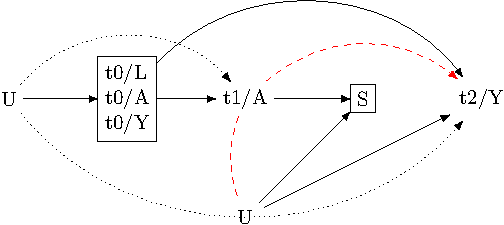
\includegraphics[width=0.8\textwidth,height=\textheight]{causal-dags_files/figure-pdf/fig-dag-8-1.pdf}

}

\caption{\label{fig-dag-8}Causal diagram of a three-wave panel design
with selection bias. The red dashed paths reveal the open backdoor path
induced by conditioning on the selected sample.}

\end{figure}

\hypertarget{unmeasured-confounder-affects-outcome-and-variable-that-affects-attrition}{%
\subsubsection{Unmeasured confounder affects outcome and variable that
affects
attrition}\label{unmeasured-confounder-affects-outcome-and-variable-that-affects-attrition}}

Figure~\ref{fig-dag-8-2} presents another problem of selection bias in a
three-wave panel design. This diagram shows how an unmeasured
confounder, U\(_S\), can simultaneously influence the outcome variable
Y\(_{t2}\) and another variable, L\(_{t2}\), responsible for attrition
(i.e., the drop-out rate, denoted as \(\framebox{S}\)). Here we present
a scenario in which the exposure variable \(A_{t1}\) can impact a
post-treatment confounder L\(_{t2}\), which subsequently affects
attrition, \(\framebox{S}\). If the study's selected sample descends
from L\(_2\), the selection effectively conditions on L\(_{t2}\),
potentially introducing bias into the analysis. Figure~\ref{fig-dag-8-2}
marks this biasing pathway with red-dashed lines. Ordering the nodes
chronologically in one's graph elucidates the assumed temporal sequence
of events, allowing for a more precise assessment of potential bias
sources relevant to a three-wave panel design.

\begin{figure}

{\centering 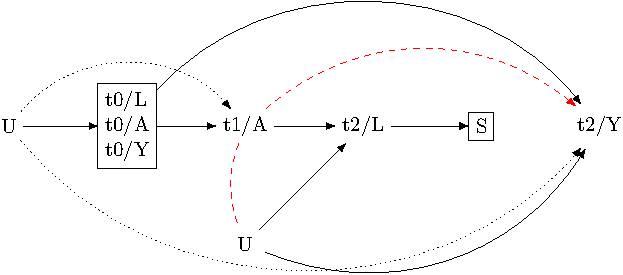
\includegraphics[width=0.8\textwidth,height=\textheight]{causal-dags_files/figure-pdf/fig-dag-8-2-1.pdf}

}

\caption{\label{fig-dag-8-2}Causal diagram of a three-wave panel design
with selection bias: example 2: Unmeasured confounder U\_S, is a cause
of both of the outcome Y\_2 and of a variable, L\_2 that affects
attrition, S. The exposure A affects this cause L\_2 of attrition, S.
The selected sample is a descendent of L\_2. Hence selection is a form
of conditioning on L\_2. Such conditioning opens a biasing path,
indicated by the red-dashed lines.}

\end{figure}

\hypertarget{why-regression-adjustment-fails-to-address-select-bias-from-attrition}{%
\subsubsection{Why regression adjustment fails to address select bias
from
attrition}\label{why-regression-adjustment-fails-to-address-select-bias-from-attrition}}

We cannot address selection bias from attrition using regression.
Shifting the example from culture to health, suppose that sicker
individuals or those with less successful outcomes are likelier to drop
out of the study. If this occurs, the remaining sample will not
represent the original population; it will over-represent healthier
individuals or those with more successful outcomes.

We use regression adjustment to control for confounding variables across
the treatment groups. With loss-to-follow-up, regression adjustment can
only address selection bias. The remaining censored population may
differ from the source population in the average association between the
exposure and the outcome.

What to do?

\begin{enumerate}
\def\labelenumi{\arabic{enumi}.}
\item
  \textbf{Prevention}: obviously, the best way to deal with missing data
  is to prevent it in the first place. Maintain regular contact with
  study participants, using incentives for continued participation,
  making follow-ups as convenient as possible, and tracking participant
  details from multiple sources (email, phone, secondary contacts).
\item
  \textbf{Missing data imputation}: this requires predicting the missing
  values based on our data, assuming that the missingness is random
  conditional on baseline measures. Note that this missingness should be
  predicted separately within strata of the exposed and unexposed in the
  previous wave (see: (\protect\hyperlink{ref-westreich2015}{Westreich
  et al. 2015}; \protect\hyperlink{ref-zhang2023}{Zhang et al. 2023})).
  Imputation methods typically assume that data are missing conditional
  on a correctly specified model and information obtained at baseline.
\item
  \textbf{Inverse probability weighting with censoring weights}: this
  requires weighting the values of each participant in the study by the
  inverse of the probability of their observed pattern of missingness
  (censoring weights)(\protect\hyperlink{ref-leyrat2019}{Leyrat et al.
  2019}; \protect\hyperlink{ref-cole2008}{Stephen R. Cole and Hernán
  2008}). In this approach, the sample gives more weight to
  under-represented individuals owing to drop-out. As with missing data
  imputation, IPW with censoring weights also assumes that we can
  correctly model the missingness from the observed data.
\item
  \textbf{Sensitivity analysis}: as with nearly all causal inference, we
  should quantitatively evaluate how sensitive results are to different
  assumptions and methods for handling censoring events
  (\protect\hyperlink{ref-shi2021}{Shi et al. 2021}).
\end{enumerate}

\hypertarget{summary-of-part-4}{%
\subsubsection{Summary of Part 4}\label{summary-of-part-4}}

In this segment, I used causal diagrams to clarify potential confounding
from selection bias. Here is my take-home advice:

\begin{enumerate}
\def\labelenumi{\arabic{enumi}.}
\item
  \textbf{Broad sampling}: to ensure that the results of your study can
  be generalised, strive to sample extensively from the target
  population. A broad sample will offer more opportunities to measure
  all effect modifiers. With these data.
\item
  \textbf{Accurate measurement and adjustment for covariates}: in
  developing a three-wave panel, addressing Type 2 selection bias
  requires precise measurements and appropriate confounding control
  (\protect\hyperlink{ref-lu2022}{Lu et al. 2022}). Failing to measure
  and adjust for these covariates may lead to erroneous conclusions
  about the relationship between exposure and outcome.
\item
  \textbf{Construct causal diagrams for the target population}: causal
  diagrams should represent confounding as it exists in the target
  population (see Suzuki, Shinozaki, and Yamamoto
  (\protect\hyperlink{ref-suzuki2020}{2020}), especially the
  supplementary materials provided).
\item
  \textbf{Maximise retention}: retention, retention, retention. Rention
  is the mission-critical objective.
\item
  \textbf{Use multiple imputation or inverse probability of treatment
  with censoring weights to adjust for attrition} Achieving a 100\%
  retention rate is typically unattainable. To reduce disparities
  between the source population at baseline and the population from
  which the censored participants were drawn.
\item
  \textbf{Perform sensitivity analyses} to assess the robustness of
  results to methods for handling attrition.
\end{enumerate}

\hypertarget{part-5.-applications-of-causal-diagrams-to-the-understanding-of-measurement-bias}{%
\subsection{Part 5. Applications of Causal Diagrams to the Understanding
of Measurement
Bias}\label{part-5.-applications-of-causal-diagrams-to-the-understanding-of-measurement-bias}}

Here we use causal diagrams to clarify bias from measurement error,
revealing implications for research design. Following Miguel A. Hernán
and Cole (\protect\hyperlink{ref-hernuxe1n2009}{2009}), we first define
structural concepts of measurement error and draw causal diagrams to
understand how they may bias causal effect estimates (see also
(\protect\hyperlink{ref-vanderweele2012}{Tyler J. VanderWeele and Hernán
2012})).

\hypertarget{uncorrelated-non-differential-undirected-measurement-error}{%
\subsubsection{1. Uncorrelated non-differential (undirected) measurement
error}\label{uncorrelated-non-differential-undirected-measurement-error}}

As shown in Figure~\ref{fig-dag-uu-null}, an uncorrelated
non-differential measurement error occurs when the errors in the
measurement of the exposure and outcome are not related.

To clarify, consider again the task of estimating the causal effect of
beliefs in Big Gods on social complexity. Suppose ancient societies
randomly omitted or recorded details about both beliefs in Big Gods and
indicators of social complexity in their records. Alternatively, suppose
that such records were not preserved equally across cultures for reasons
unrelated to these parameters. In this case, errors in the documentation
of both variables would be random. The errors would not be related to
the intensity of the beliefs in Big Gods or the level of social
complexity. This example of uncorrelated and non-differential error is
presented in Figure~\ref{fig-dag-uu-null}.

Uncorrelated non-differential measurement error does not create bias
under the null. As evident from Figure~\ref{fig-dag-uu-null},
d-separation is preserved. Equivalently, there are no open backdoor
paths on the graph. However, when there is an actual effect of the
exposure on the outcome, non-differential measurement error generally
leads to attenuated effect estimates. For this reason, uncorrelated
non-differential measurement error can be problematic for inference even
though it does not induce structural bias under the null.

\begin{figure}

{\centering 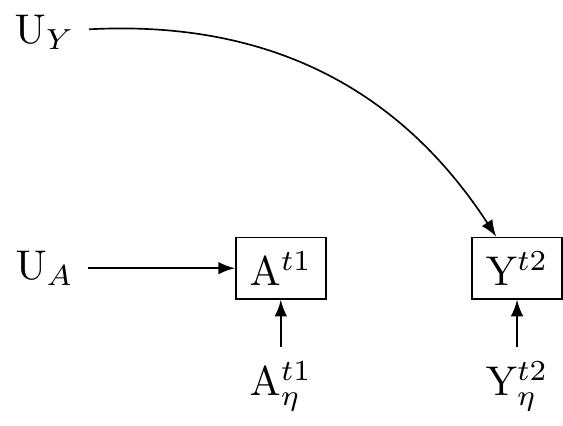
\includegraphics[width=0.6\textwidth,height=\textheight]{causal-dags_files/figure-pdf/fig-dag-uu-null-1.pdf}

}

\caption{\label{fig-dag-uu-null}Uncorrelated non-differential
measurement error does not bias estimates under the null, however may
attenuate true effects.}

\end{figure}

\hypertarget{uncorrelated-differential-directed-measurement-error}{%
\subsubsection{2. Uncorrelated differential (directed) measurement
error}\label{uncorrelated-differential-directed-measurement-error}}

As shown in Figure~\ref{fig-dag-indep-d-effect}, uncorrelated
differential (or directed) measurement error occurs when the measurement
errors are related to the level of exposure or outcome but not to each
other. For instance, societies with stronger `beliefs in Big Gods' might
have more or less detailed records of `social complexity'. Suppose that,
in the absence of any intervention on beliefs in Gods, there is no
association between the measurement errors. Here, the errors are
differential as they depend on the intensity of religious beliefs but
are uncorrelated as the errors in documenting `beliefs in Big Gods' and
`social complexity' are otherwise independent. Uncorrelated differential
(or directed) measurement error is presented in
Figure~\ref{fig-dag-indep-d-effect} and leads to bias under the null,
indicated by the red path. Alternatively, equivalently, uncorrelated
differential (or directed) measurement error opens a backdoor path
between the exposure and the outcome.

Note that the bias presented in Figure~\ref{fig-dag-indep-d-effect}, an
example of directed measurement error, also describes the bias we
considered when there is panel attrition and which the exposure affects
selection (see: Figure~\ref{fig-dag-8-5}). In that scenario, the outcome
in the selected group is measured with error -- it no longer represents
the measurement of the outcome in the source population at baseline --
furthermore, this error is affected by exposure. The previous example
described bias in estimation from the vantage point of collider
stratification; however, we can also explain the distortion as directed
measurement bias.

\begin{figure}

{\centering 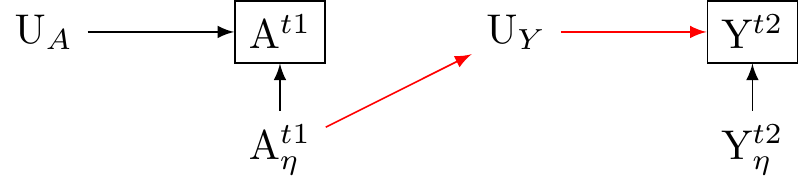
\includegraphics[width=1\textwidth,height=\textheight]{causal-dags_files/figure-pdf/fig-dag-indep-d-effect-1.pdf}

}

\caption{\label{fig-dag-indep-d-effect}Directed independent
(uncorrelated) measurement error can bias effect estimates under the
null. This bias is indicated by the red path.}

\end{figure}

\hypertarget{correlated-non-differential-undirected-measurement-error}{%
\subsubsection{3. Correlated non-differential (undirected) measurement
error}\label{correlated-non-differential-undirected-measurement-error}}

As shown, Figure~\ref{fig-dag-dep-u-effect} correlated non-differential
(undirected) measurement error occurs when the errors in measuring both
the exposure and outcome are related independently of the exposure. The
scenario is presented in Figure~\ref{fig-dag-dep-u-effect}. Imagine that
some societies had more advanced record-keeping systems that resulted in
more accurate and detailed accounts of both beliefs in Big Gods and
social complexity. Furthermore, imagine that record keepers provide
better information about religious beliefs. In this case, the errors
between beliefs in Big Gods and social complexity are correlated because
the accuracy of records for both variables is influenced by the same
underlying factor (the record-keeping abilities). However, the errors
are not directed insofar as levels of religious beliefs and social
complexity do not affect the assumed bias in record keeping. Correlated
non-differential measurement error may induce bias under the null,
indicated by the red path in Figure~\ref{fig-dag-dep-u-effect}.

\begin{figure}

{\centering 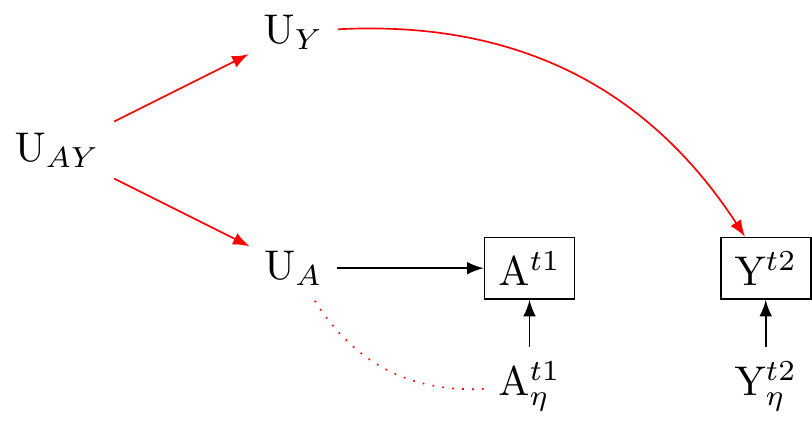
\includegraphics[width=0.8\textwidth,height=\textheight]{causal-dags_files/figure-pdf/fig-dag-dep-u-effect-1.pdf}

}

\caption{\label{fig-dag-dep-u-effect}Correlated undirected measurement
error can distort causal effect estimates under the null, indicated by
the red path.}

\end{figure}

\hypertarget{correlated-differential-directed-measurement-error}{%
\subsubsection{4. Correlated differential (directed) measurement
error}\label{correlated-differential-directed-measurement-error}}

Correlated differential (directed) measurement error occurs when the
measurement errors are related independently of the exposure, and the
exposure also affects levels of these correlated error terms. The
structure of this bias is presented in Figure~\ref{fig-dag-d-d}. Suppose
societies with stronger beliefs in Big Gods tend to record their
religious beliefs and social structures more meticulously than others.
Suppose further that religious elites conduct this record-keeping. The
errors may be both correlated and differential if societies with beliefs
in Big Gods tend to favour these religious elites, leading to biased
records.

Consider further the three-wave panel design, where we aim to estimate
the effect of self-reported religious service attendance on
self-reported monthly donations to charity. A set of confounders is
included at baseline, comprising previous measures of religious service
attendance and monthly donations to charity. Because our measures rely
on self-reports, they may be especially prone to measurement error.

Assume there is an unmeasured common cause affecting both the
measurement error of religious service attendance and the measurement
error of donations to charity. This bias might occur if individuals
consistently over- or under-report their religious service attendance
and donations due to social desirability bias.

In Part 3, we discussed how including the exposure measured at baseline
can reduce confounding in a three-wave panel design. By controlling for
the baseline exposure, we effectively adjust for any static
characteristics that cause a correlation between the exposure and
outcome.

Now for measurement error, including baseline measures could mitigate
the impact of these errors on causal effect estimation, provided the
errors are random and not systematically associated across time points.

To see this, let \(A_0\), \(A_1\) denote the exposure at baseline and
follow-up, and \(Y_0\), \(Y_1\) denote the outcome at baseline and
follow-up. The true values are denoted without primes, and the measured
values are with primes. We assume the measurement error is additive:

\(A'_0 = A_0 + UA_0\),

\(A'_1 = A_1 + UA_1\),

\(Y'_0 = Y_0 + UY_0\),

\(Y'_2 = Y_2 + UY_2\),

where \(UA_0\), \(UA_1\) are the measurement errors for the exposure at
baseline and follow-up, and \(UY_0\), \(UY_2\) are the measurement
errors for the outcome at baseline and follow-up. If the errors are
correlated, then \(Cov(UA_0, UY_0) \neq 0\) and/or
\(Cov(UA_1, UY_2) \neq 0\).

In a model that includes \(A'_0\) and \(Y'_0\) as covariates, the
estimated effect of \(A'_1\) on \(Y'_2\) identifies the effect of change
in the exposure from baseline to follow-up on the incidence effect.
Because our interest is in this incidence effect, we control for the
baseline exposure and outcome measures. This strategy will mitigate bias
arising from correlated errors if the following conditions hold:

\(E(UA_0) = E(UA_1)\) and \(E(UY_0) = E(UY_2)\) (i.e., the expectation
of the measurement errors does not change over time),

\(Cov(UA_0, UY_2) = Cov(UA_1, UY_2)\) (i.e., the correlation between the
errors does not change over time).

Thus, including baseline measurements in our model can mitigate
undirected measurement errors. However, this solution hinges on the
measurement error being undirected and non-differential concerning time.
If the measurement error varies over time or affects other variables in
the model, baseline measurement control will be inadequate for
confounding control (see: (\protect\hyperlink{ref-keogh2020}{Keogh et
al. 2020})).

Consider a scenario where individuals who attend religious service more
at wave 1 acquire more substantial social desirability bias, becoming
more likely to over-report socially desirable behaviours or under-report
socially undesirable ones. The structure of this scenario is presented
in Figure~\ref{fig-dag-d-d}. If the measured outcome at wave 2 is
charitable giving, the increased social desirability bias could lead to
an overestimation of the actual level of giving. Suppose we compare
reported charity at wave 2 with reported religious attendance at wave 1.
If there is directed measurement bias we might falsely attribute the
apparent increase in charity to the increase in religious service
attendance, when, in reality, there was over-reporting from social
desirability bias that was induced by religious service attendance. Here
we can see that if the error of the outcome is affected by the exposure,
the causal effect of the increase in religious service on charitable
giving might be different from the association presented in the data.

Thus, although controlling for baseline exposure is a powerful strategy
for isolating incidence effects and controlling confounding, we have
seen that it is not a catch-all solution. Attention to the quality of
measures at all time points remains critical.

For instance, to avoid presentation bias, rather than asking whether one
has \emph{offered} help, we might ask participants in a multi-wave study
whether they have \emph{received help} -- under the assumption that if
the religious community is more altruistic than the secular community,
the probability of receiving help will be higher.

\begin{figure}

{\centering 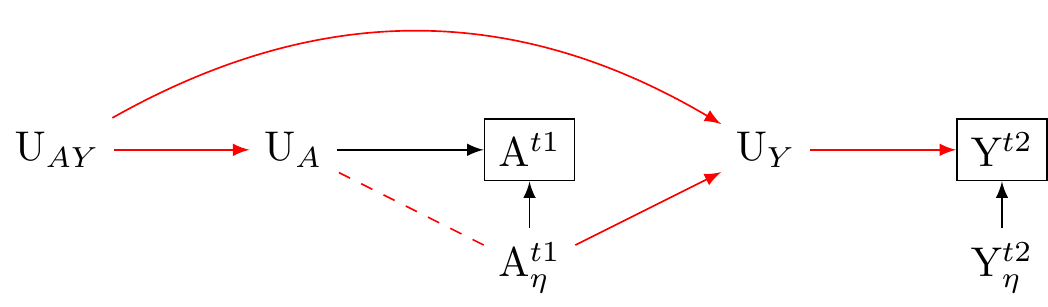
\includegraphics[width=1\textwidth,height=\textheight]{causal-dags_files/figure-pdf/fig-dag-d-d-1.pdf}

}

\caption{\label{fig-dag-d-d}Directed dependent (correlated) measurement
error leads to bias in effect estimates. Here, the exposure affects the
measurement error of the outcome. Additionally, the measurement error of
the exposure and outcome are correlated. These dynamics open pathways
for bias, indicated by the red paths.}

\end{figure}

\hypertarget{correlated-undirected-measurement-error-in-comparative-cultural-research}{%
\subsubsection{Correlated undirected measurement error in comparative
cultural
research}\label{correlated-undirected-measurement-error-in-comparative-cultural-research}}

In comparative cultural research, a common practice is to use invariance
testing, a set of statistical models, to evaluate the appropriateness of
the measures employed. However, statistical models do not determine
structural models: statistical tests performed on cross-sectional
datasets may not effectively identify causal features.

How might we understand those causal features?
Figure~\ref{fig-dag-dep-u-effect-selection} shows how selecting study
participants from different cultures that systematically differ in their
responses to the exposure and outcome may induce correlated measurement
errors. To show this possibility, we adjust the causal diagram presented
as Figure~\ref{fig-dag-dep-u-effect} and incorporate the selection into
the study. The resulting graph is presented in
Figure~\ref{fig-dag-dep-u-effect-selection}.

If we were to select participants from a setting devoid of systematic
(correlated) error structures between the exposure and outcome
measurements, we might avoid such confounding. However, the very process
of sample selection in a cross-cultural study may open pathways for
measurement bias if people from different cultures interpret and respond
to the measures differently. We cannot stratify on culture to address
the problem because stratifying on culture is what evokes correlated
measurement error.

\begin{figure}

{\centering \includegraphics[width=1\textwidth,height=\textheight]{causal-dags_files/figure-pdf/fig-dag-dep-u-effect-selection-1.pdf}

}

\caption{\label{fig-dag-dep-u-effect-selection}Measurement bias in
comparative cross-cultural research. Selection at baseline induces
correlations in the measurement error of the exposure and outcome.
Biasing paths are presented in red.}

\end{figure}

\hypertarget{using-causal-diagrams-to-clarify-the-structural-assumptions-of-latent-factor-models}{%
\subsubsection{Using causal diagrams to clarify the structural
assumptions of latent factor
models}\label{using-causal-diagrams-to-clarify-the-structural-assumptions-of-latent-factor-models}}

Cultural evolution researchers who wish to record cultural evolutionary
dynamics in the present may consider using multi-item constructs in
their panel studies. Multi-item constructs have long been favoured by
traditional psychometric theory. However, classical psychometric theory
developed without the benefit of causal approaches. VanderWeele argues
that difficulties surface when assessing the causal assumptions of
formative and reflective latent factor models
(\protect\hyperlink{ref-vanderweele2022}{Tyler J. VanderWeele 2022}).
These models are based on statistical formulations. However, the causal
inferences they embody cannot be determined solely by statistical
models. This discussion will concentrate on reflective models, although
the concerns raised are equally applicable to formative models, and I
refer interested readers to:
(\protect\hyperlink{ref-vanderweele2022}{Tyler J. VanderWeele
2022}).\footnote{In formative models, observed variables are perceived
  to generate the latent variable. This latent variable is assumed to be
  a composite of the observed variables, \(X_i\), mathematically
  expressed as \(\eta = \sum_i\lambda_i X_i\). The structural assumption
  is that a single latent variable causally influences the observed
  variables. This structural is depicted in
  Figure~\ref{fig-structural-assumptions-reflective-model}.}

\begin{figure}

{\centering 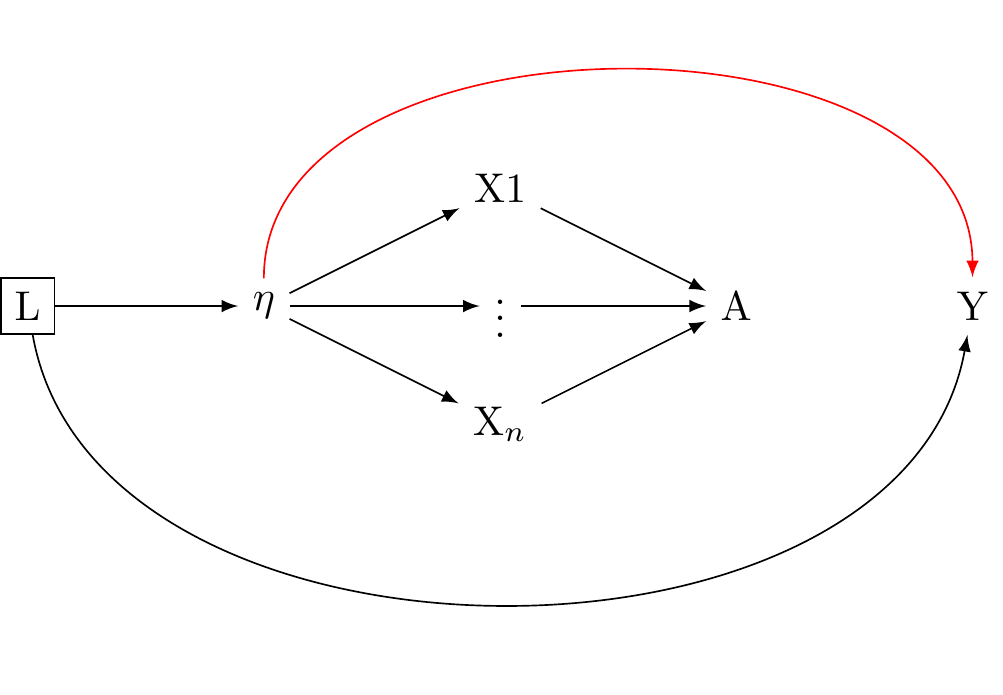
\includegraphics[width=0.8\textwidth,height=\textheight]{causal-dags_files/figure-pdf/fig-structural-assumptions-reflective-model-1.pdf}

}

\caption{\label{fig-structural-assumptions-reflective-model}Structural
assumptions of the reflective model imply a univariate reality causes
the outcome. These assumptions are strong because they exclude
multivariate causes of the indicators for constructs, as well as
independent effects of the indicators on outcomes. The figure is adapted
from VanderWeele: doi: 10.1097/EDE.0000000000001434}

\end{figure}

However, VanderWeele notes that the statistical model is consistent with
multiple causal models. The presumption that a univariate latent reality
underlies the reflective (and formative) latent factor models is a
stronger assumption than previously acknowledged. For example, an
alternative structural model equally compatible with the data is
presented in Figure~\ref{fig-dag_multivariate_reality_again}. Here,
multivariate reality gives rise to the indicators from which we draw our
measures. Indeed, for specific widely used measures, the assumption of a
univariate reality is so strong that they make testable assumptions, and
empirical examination of these assumptions reveals the tests fail
(\protect\hyperlink{ref-vanderweele2022b}{Tyler J. VanderWeele and
Vansteelandt 2022}). Although we cannot determine which structural model
is accurate, the data rule out the univariate model.

\begin{figure}

{\centering \includegraphics[width=0.6\textwidth,height=\textheight]{causal-dags_files/figure-pdf/fig-dag_multivariate_reality_again-1.pdf}

}

\caption{\label{fig-dag_multivariate_reality_again}Vanderweele's example
of an alternative structural model that is consistent with the
statistical model that underpins reflective construct models. Here, a
multivariate reality gives rise to the indicators from which we draw our
measures. The figure is adapted from VanderWeele: doi:
10.1097/EDE.0000000000001434}

\end{figure}

Although the assumptions of a univariate reality that underlie
traditional latent factor models are not generally credible, VanderWeele
suggests that construct measures can still find application in research.
The key to salvaging latent factor models is to extend the theory of
causal inference under multiple interventions to latent factor models
(\protect\hyperlink{ref-vanderweele2022}{Tyler J. VanderWeele 2022}).
Specifically, by framing measured variables as functions of indicators
that may map onto a complex multivariate underlying reality, we may
approach them as coarsened indicators for that reality. As long as the
potential outcomes of these coarsened indicators are conditionally
independent of their treatment assignments and there is no unmeasured
confounding, we may assume the constructs to consistently estimate the
causal effects of the complex reality that gives rise to them. This
interpretation is presented in
Figure~\ref{fig-dag-multiple-version-treatment-applied-measurement}.
Just as with the theory of causal inference under multiple versions of
treatments, there may be circumstances where ensuring conditional
exchangeability is unattainable; even when such assurance is feasible,
interpreting the results or advocating policy intervention may be
problematic. Thus, I maintain a more restrained optimism about this
generalisation of the theory of causal inference under multiple versions
of treatment. In the subsequent section, I show how a causal diagram
helps to clarify the unresolved measurement biases.

\begin{figure}

{\centering 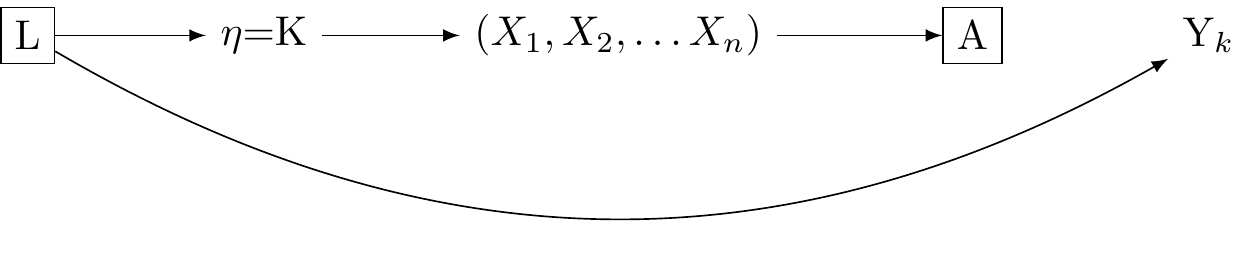
\includegraphics[width=0.8\textwidth,height=\textheight]{causal-dags_files/figure-pdf/fig-dag-multiple-version-treatment-applied-measurement-1.pdf}

}

\caption{\label{fig-dag-multiple-version-treatment-applied-measurement}Vanderweele's
solution: the theory of causal inference under multiple versions of
treatment may be applied to measurement models. The indicators used in
constructs may map onto a complex multivariate reality if each element
of the approach is a coarsened indicator that is conditionally
independent of the outcome. The figure is adapted from VanderWeele: doi:
10.1097/EDE.0000000000001434}

\end{figure}

\hypertarget{causal-diagrams-highlight-issues-arising-from-measurement-errors-within-construct-components}{%
\subsubsection{Causal diagrams highlight issues arising from measurement
errors within construct
components}\label{causal-diagrams-highlight-issues-arising-from-measurement-errors-within-construct-components}}

Consider a three-wave panel with the assumption that no unmeasured
confounding exists. We represent the exposure \(A\) as a function of
indicators, \(A_{f(A_1, A_2, ..., A_n)}\), representing a coarsened
state of a multivariate reality. Each component of this reality
corresponds to a structural element, represented as
\(\eta_{A_1}, \eta_{A_2}, ..., \eta_{A_n}\), each with associated error
terms, \(U\eta_{A_1}, U\eta_{A_2}, ..., U\eta_{A_n}\).

We can similarly conceptualise the outcome \(Y\), as a function of
indicators, \(Y_{f(Y_1, Y_2, ..., Y_n)}\), representing a latent
reality. This latent reality is composed of the components
\(\eta_{Y_1}, \eta_{Y_2}, ..., \eta_{Y_n}\), each with their
corresponding error terms
\(U\eta_{Y_1}, U\eta_{Y_2}, ..., U\eta_{Y_n}\).

Figure~\ref{fig-dag-coarsen-measurement-error} depicts this assumed
reality and outlines potential confounding paths due to directed
measurement error. Each path consists of a structural component
\(\eta_{A_n}\) and its associated error term \(U\eta_{Y_n}\). We
identify three potential confounding paths resulting from directed
measurement error.

The potential for confounding from measurement error in panel designs
fundamentally relies on the relationships and dependencies among
variables, not their quantity. However, it is worth emphasising that, in
theory, an increase in the number of latent states or error terms could
enhance the potential for confounding. Under simplifying assumptions,
the potential direct paths from the exposure to the outcome are given by
the product of the number of components of the exposure and the number
of error terms associated with the outcome, symbolically represented as
\(\eta A_n \times U\eta_{Y_n}\). In this simplified scenario, each
latent variable connected to exposure could influence every error term
of an outcome, creating a complex network of confounding paths.

Causal diagrams applied to measurement error in latent factor models
reveal the importance of rigorously considering construct measures in
evolutionary and other human sciences. Although there is no universal
rule here, researchers might sometimes opt to use single-item measures.
Each case, however, demands a meticulous examination of the items'
meanings, probable interpretations, and potential causal implications
over time.

\begin{figure}

{\centering 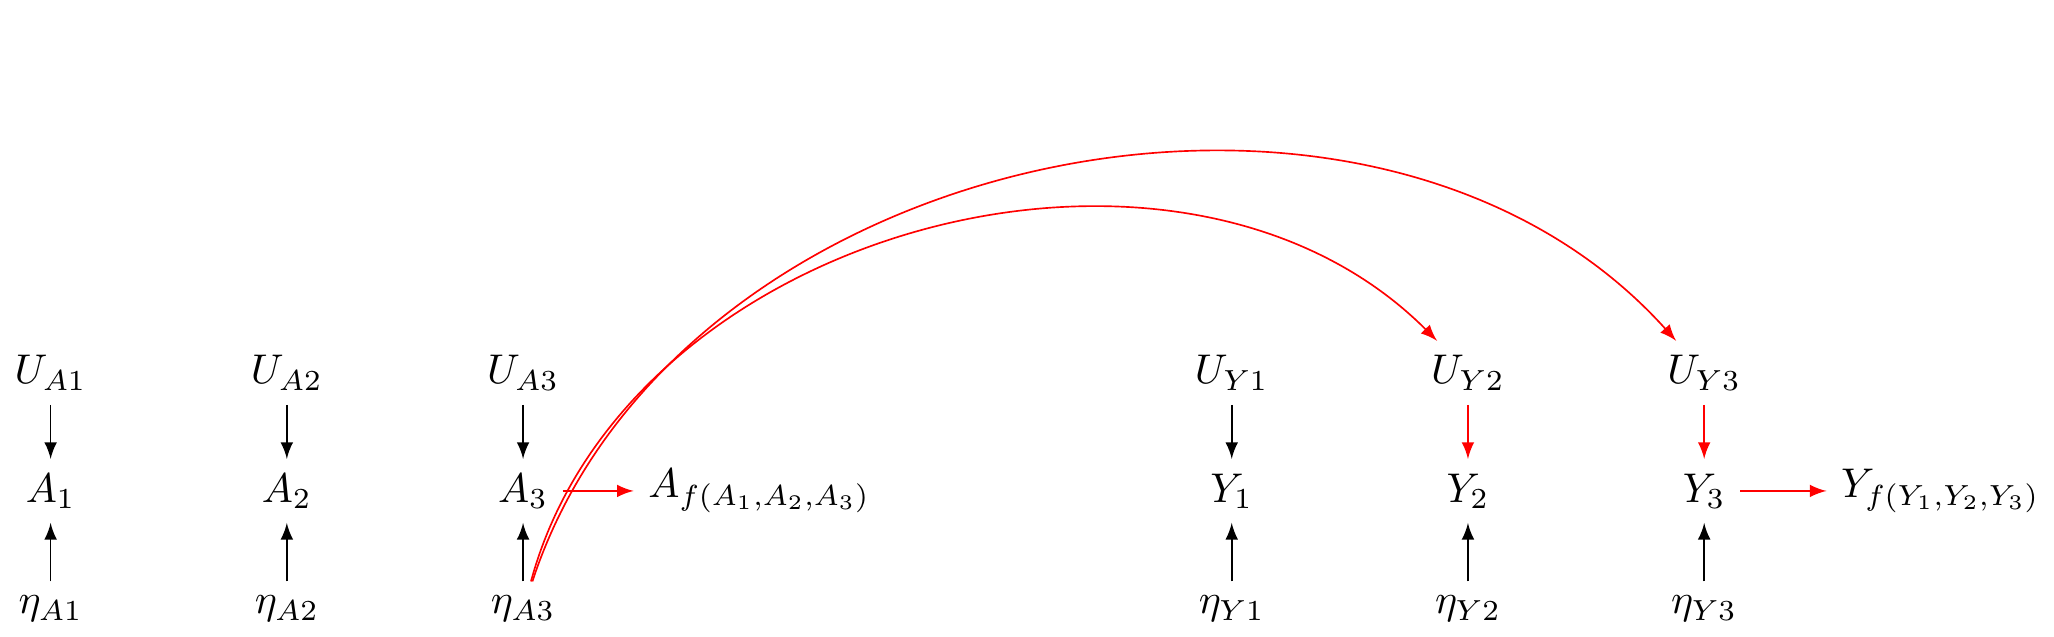
\includegraphics[width=1\textwidth,height=\textheight]{causal-dags_files/figure-pdf/fig-dag-coarsen-measurement-error-1.pdf}

}

\caption{\label{fig-dag-coarsen-measurement-error}Where there are many
indicators of a psychological construct, there are many opportunities
for additional confounding by directed measurement error.}

\end{figure}

\hypertarget{summary-part-5}{%
\subsubsection{Summary Part 5}\label{summary-part-5}}

Part 5 has centred on clarifying the biases that measurement error
brings to the repeated measures designs. Such designs are typically
necessary for the quantitative estimation of causal effects. I have
examined four kinds of measurement error, assessing how each might skew
inference. While adjustments for baseline exposure can aid in reducing
confounding and isolating incidence effects, it is not a panacea for all
biases. A researcher must meticulously scrutinise the quality of
measurements at all time points, assessing and averting potential
biases.

Although methods for adjusting for measurement error are not covered in
this article, a host of useful resources exists, including the works of
Keogh et al. (\protect\hyperlink{ref-keogh2020}{2020}) Buonaccorsi
(\protect\hyperlink{ref-buonaccorsi2010}{2010}) Shi et al.
(\protect\hyperlink{ref-shi2021}{2021}) Valeri, Lin, and VanderWeele
(\protect\hyperlink{ref-valeri2014}{2014}) and Bandalos
(\protect\hyperlink{ref-bandalos2018}{2018}).

\hypertarget{review}{%
\subsubsection{Review}\label{review}}

Should Cicero have been present in our era, he might exclaim:
``\emph{Causalis Ante Statisticum!}'' --- prioritise the causal over the
statistical!

In the human sciences, statistical models hold sway. This interest is
understandable. Statistics is indispensable for quantitative insights.
However, wherever we aim to understand the effects of interventions
quantitatively, a structural approach take precedence. Statistics come
later.

Causal analysis requires a well-defined exposure and outcome that are
accurately measured. Establishing the chronological sequence of these
variables on a timeline is vital for this accuracy. Additionally, it
requires an expert assessment of any factors that could link these
variables independent of causation. For such confounding parameters and
their proxies, meticulous measurements must also be taken, and their
chronological order relative to the exposure and outcome must be clear.
Next, sequential measurements of the exposure, followed by the outcomes,
should be conducted on enough units to emulate a well-powered target
trial.

When comparing outcomes across exposed and unexposed units, typically
individuals, a rigorous follow-up and retention effort is needed.
Tracking individuals is difficult. Given the inevitability of retention
failures in any sizeable sample, counteracting biases from loss to
follow-up forms a vital part of the work. There are no shortcuts.

Nearly all of the work in causal inference extends beyond merely fitting
models to data -- although it is undoubtedly that too. Moreover, the
statistical models that robust counterfactual data science demands,
which I have not covered in this article, are complex. Causal inference,
then, is a labour of love. This labour is not for the faint-hearted.
Nonetheless, it is worth the effort because it offers hope for a
quantitative understanding of the causal effects of interventions. Such
an understanding animates the curiosity and drive of most human
scientists, even if we have too often contented ourselves with
correlations. (For many years, I was such a human scientist.) In this
discussion, I have described several ways that chronologically ordered
causal diagrams significantly contribute to causal inference, or what I
have termed ``counterfactual data science.'' Their utility is not
limited to modelling; they are excellent guides for data collection.
With judicious use, causal diagrams can aid our quest for the robust
causal understanding we seek.

\hypertarget{summary-of-advice}{%
\subsubsection{Summary of advice}\label{summary-of-advice}}

\begin{enumerate}
\def\labelenumi{\arabic{enumi}.}
\item
  \textbf{Clearly define all variables}: define your exposure and
  outcome through protocols of a hypothetical experiment or ``target
  trial.''
\item
  \textbf{Clearly define novel conventions}: if you use unique
  conventions in your diagram -- such as coloured or dash edges --
  ensure the conventions are clearly defined.
\item
  \textbf{Ensure the graph is acyclic}: nodes cannot be their own
  ancestors.
\item
  \textbf{Time-stamp nodes}: time-stamping nodes often provide clearer
  temporal understanding. Because causation occurs in time, causal
  diagrams benefit if this understanding is visually evident.
\item
  \textbf{Maintain chronological order}: arrange nodes in temporal
  sequence, generally from left to right or top to bottom.
\item
  \textbf{Embrace minimalism}: include only those essential nodes and
  edges for clarifying the identification problem. Refrain from
  cluttering the causal diagram. The sequence of events should be
  evident in the spatial layout. However, it is rarely necessary to draw
  that sequence to scale.
\item
  \textbf{Show vectors for unmeasured confounding} : plan for
  sensitivity analyses to assess whether unmeasured confounding might
  explain away the results.
\item
  \textbf{Show nodes for post-treatment selection}: this helps to
  understand potential sources of selection bias.
\item
  \textbf{Should mediation or interaction be of interest, extend the
  graphs to clarify the relevant structures of bias}: Do not attempt to
  draw non-linear associations between the variables.
\item
  \textbf{Appreciate causal diagrams are qualitative tools that encode
  assumptions about causal ancestries}: causal diagrams are akin to
  compasses that guide us to close backdoor paths. We should refrain
  from using them as exhaustive atlases.
\item
  \textbf{Show vectors of correlated and/or directed measurement error}:
  where such vectors may be assumed to create compromising bias.
\item
  \textbf{Note, causal diagrams are structural models; structural
  equation models are not structural models}: ``structural'' meands
  causal. Structural equation modelling is essentially a statistical
  exercise. The coefficients it generates can often be challenging to
  interpret in causal terms. Regression coefficients, including those of
  structural equation modelling, rarely afford causal interpretations.
  If our interest is in causal inference, we should generally avoid
  reporting them -- they typically have no meaning. In our discussion of
  mediation and treatment-confounder feedback, we considered the
  complexities that arise for causal inferences in what would appear to
  be simple scenarios. G-methods offer robust strategies for causal
  estimation that can address complex longitudinal questions involving
  multiple and sequential exposures. Despite their potency, G-methods
  still need to be utilised in fields such as cultural evolution. If
  there is more than one exposure event such that exposure can affect
  the confounders of the next exposure event, or such that a hidden
  confounder can relate them, we must (presently) use G-methods.
\end{enumerate}

\hypertarget{concluding-remarks}{%
\subsubsection{Concluding remarks}\label{concluding-remarks}}

Causal inference is vital for science because it offers a way to
quantify the effects of interventions. However, it is only a small part
of science. Particularly in the historical sciences, the fundamental
assumptions of causal inference may not be applicable. We should not
abandon sciences that do not quantify causal effect estimates.

That said, many human scientists have yet to adopt causal inferential
approaches. In most fields, the correlational methods that have held
sway, at least since Karl Pearson, still hold sway. We are a long way
from overstating the importance of causal inference.

Chronologically ordered causal diagrams clarify why time-series data are
indispensable for addressing quantitative causal questions. The nearly
absolute requirement for time-series data collection for causal
inference carries profound implications for research design, funding
models, and the pace of scientific discovery. Given the time for
research preparation, data collection, and data entry, a three-year
panel design will require at least five years of support. Existing
funding models often extend only 2-3 years. Researchers who seek causal
understanding and their funders must exhibit patience. How many will
support the patience science that causal inference demands? The present
funding models across the human sciences have yet to offer it. (Although
I am fortunate to have been an exception.)

Most human scientists want to understand the effects of interventions on
the world. Progress depends on our ability to transition from a
productivity model of human science reminiscent of an assembly line or
counterfeit money press to a system that nurtures long-term data
collection.

\newpage{}

\hypertarget{appendix-1-review-of-vanderweeles-theory-of-causal-inference-under-multiple-versions-of-treatment}{%
\subsection{Appendix 1: Review of VanderWeele's theory of causal
inference under multiple versions of
treatment}\label{appendix-1-review-of-vanderweeles-theory-of-causal-inference-under-multiple-versions-of-treatment}}

We denote an average causal effect as the change in the expected
potential outcomes when all units receive one level of treatment
compared to another.

Let \(\delta\) denote the causal estimand on the difference scale
\((\mathbb{E}[Y^1 - Y^0])\). The causal effect identification can be
expressed as:

\[ \delta = \sum_l \left( \mathbb{E}[Y|A=a,l] - \mathbb{E}[Y|A=a^*,l] \right) P(l)\]

The theory of causal inference with multiple treatment versions provides
a conceptual framework for causal inference in observational studies.
Suppose we can assume that for each treatment version, the outcome under
that version equals the observed outcome when that version is
administered, conditional on baseline covariates and satisfaction of
other assumptions. In that case, we can consistently estimate causal
contrasts, even when treatments vary.

This approach interprets treatment indicator \(A\) as multiple actual
treatment versions \(K\). Furthermore, if we can assume conditional
independence, meaning there is no confounding for the effect of \(K\) on
\(Y\) given \(L\), we have: \(Y(k)\coprod A|K,L\).

This condition implies that, given \(L\), \(A\) adds no additional
information about \(Y\) after accounting for \(K\) and \(L\). If
\(Y = Y(k)\) for \(K = k\) and \(Y(k)\) is independent of \(K\),
conditional on \(L\), we can interpret \(A\) as a simplified indicator
of \(K\). This scenario is depicted in
Figure~\ref{fig-dag_multiple_version_treatment_dag}.

With the necessary assumptions in place, we can derive consistent causal
effects. The causal effect can be expressed

\[ \delta = \sum_{k,l} \left( \mathbb{E}[Y(k)|l] P(k|a,l) P(l) - \mathbb{E}[Y(k)|l] P(k|a^*,l) P(l) \right) \]

This setup is akin to a randomised trial where individuals, stratified
by covariate \(L\), are assigned a treatment version \(K\). This
assignment comes from the distribution of \(K\) for the
\((A = 1, L = l)\) subset. The control group receives a randomly
assigned \(K\) version from the \((A = 0, L = l)\) distribution.

\begin{figure}

{\centering \includegraphics[width=1\textwidth,height=\textheight]{causal-dags_files/figure-pdf/fig-dag_multiple_version_treatment_dag-1.pdf}

}

\caption{\label{fig-dag_multiple_version_treatment_dag}Causal inference
under multiple versions of treatment. Here, (A) may be regarded as a
coarseneed indicator of (K)}

\end{figure}

This theory of causal inference under multiple versions of treatment is
advantageous when treatments exhibit significant variability
(\protect\hyperlink{ref-vanderweele2013}{Tyler J. VanderWeele and Hernan
2013}). In Part 5, I explored VanderWeele's application of this theory
(which he developed) to latent factor models, where the presumption of a
single underlying reality for the items that constitute constructs can
be challenged (\protect\hyperlink{ref-vanderweele2022}{Tyler J.
VanderWeele 2022}). Furthermore, I acknowledged additional complications
not addressed by this theory extension arising from measurement error.
Specifically, the possibility that directed or correlated error terms
for the exposure and outcome could undermine inference.

\newpage{}

\hypertarget{references}{%
\subsection*{References}\label{references}}
\addcontentsline{toc}{subsection}{References}

\hypertarget{refs}{}
\begin{CSLReferences}{1}{0}
\leavevmode\vadjust pre{\hypertarget{ref-bandalos2018}{}}%
Bandalos, Deborah L. 2018. \emph{Measurement Theory and Applications for
the Social Sciences}. Guilford Publications.

\leavevmode\vadjust pre{\hypertarget{ref-bareinboim2022}{}}%
Bareinboim, Elias, Jin Tian, and Judea Pearl. 2022. {``Recovering from
Selection Bias in Causal and Statistical Inference.''} In, 1st ed.,
36:433450. New York, NY, USA: Association for Computing Machinery.
\url{https://doi.org/10.1145/3501714.3501740}.

\leavevmode\vadjust pre{\hypertarget{ref-barrett2021}{}}%
Barrett, Malcolm. 2021. \emph{Ggdag: Analyze and Create Elegant Directed
Acyclic Graphs}. \url{https://CRAN.R-project.org/package=ggdag}.

\leavevmode\vadjust pre{\hypertarget{ref-basten2013}{}}%
Basten, Christoph, and Frank Betz. 2013. {``Beyond Work Ethic: Religion,
Individual, and Political Preferences.''} \emph{American Economic
Journal: Economic Policy} 5 (3): 67--91.
\url{https://doi.org/10.1257/pol.5.3.67}.

\leavevmode\vadjust pre{\hypertarget{ref-becker2016}{}}%
Becker, Sascha O, Steven Pfaff, and Jared Rubin. 2016. {``Causes and
Consequences of the Protestant Reformation.''} \emph{Explorations in
Economic History} 62: 125.

\leavevmode\vadjust pre{\hypertarget{ref-breskin2020}{}}%
Breskin, Alexander, Andrew Edmonds, Stephen R Cole, Daniel Westreich,
Jennifer Cocohoba, Mardge H Cohen, Seble G Kassaye, et al. 2020.
{``G-Computation for Policy-Relevant Effects of Interventions on
Time-to-Event Outcomes.''} \emph{International Journal of Epidemiology}
49 (6): 2021--29. \url{https://doi.org/10.1093/ije/dyaa156}.

\leavevmode\vadjust pre{\hypertarget{ref-bulbulia2022}{}}%
Bulbulia, Joseph A. 2022. {``A Workflow for Causal Inference in
Cross-Cultural Psychology.''} \emph{Religion, Brain \& Behavior} 0 (0):
1--16. \url{https://doi.org/10.1080/2153599X.2022.2070245}.

\leavevmode\vadjust pre{\hypertarget{ref-bulbulia2021}{}}%
Bulbulia, Joseph, Uffe Schjoedt, John H Shaver, Richard Sosis, and
Wesley J Wildman. 2021. {``Causal Inference in Regression: Advice to
Authors.''} \emph{Religion, Brain \& Behavior} 11 (4): 353360.

\leavevmode\vadjust pre{\hypertarget{ref-buonaccorsi2010}{}}%
Buonaccorsi, John P. 2010. \emph{Measurement Error: Models, Methods, and
Applications}. New York: Chapman; Hall/CRC.
\url{https://doi.org/10.1201/9781420066586}.

\leavevmode\vadjust pre{\hypertarget{ref-chatton2020}{}}%
Chatton, Arthur, Florent Le Borgne, Clémence Leyrat, Florence
Gillaizeau, Chloé Rousseau, Laetitia Barbin, David Laplaud, Maxime
Léger, Bruno Giraudeau, and Yohann Foucher. 2020. {``G-Computation,
Propensity Score-Based Methods, and Targeted Maximum Likelihood
Estimator for Causal Inference with Different Covariates Sets: A
Comparative Simulation Study.''} \emph{Scientific Reports} 10 (1): 9219.
\url{https://doi.org/10.1038/s41598-020-65917-x}.

\leavevmode\vadjust pre{\hypertarget{ref-cinelli2022}{}}%
Cinelli, Carlos, Andrew Forney, and Judea Pearl. 2022. {``A Crash Course
in Good and Bad Controls.''} \emph{Sociological Methods \& Research},
May, 00491241221099552. \url{https://doi.org/10.1177/00491241221099552}.

\leavevmode\vadjust pre{\hypertarget{ref-cole2008}{}}%
Cole, Stephen R., and Miguel A. Hernán. 2008. {``Constructing inverse
probability weights for marginal structural models.''} \emph{American
Journal of Epidemiology} 168 (6): 656--64.
\url{https://doi.org/10.1093/aje/kwn164}.

\leavevmode\vadjust pre{\hypertarget{ref-cole2010}{}}%
Cole, Stephen R, Robert W Platt, Enrique F Schisterman, Haitao Chu,
Daniel Westreich, David Richardson, and Charles Poole. 2010.
{``Illustrating Bias Due to Conditioning on a Collider.''}
\emph{International Journal of Epidemiology} 39 (2): 417--20.
\url{https://doi.org/10.1093/ije/dyp334}.

\leavevmode\vadjust pre{\hypertarget{ref-collinson2007}{}}%
Collinson, Patrick. 2007. \emph{The Reformation: A History}. Vol. 19.
Modern Library.

\leavevmode\vadjust pre{\hypertarget{ref-decoulanges1903}{}}%
De Coulanges, Fustel. 1903. \emph{La Cité Antique: Étude Sur Le Culte,
Le Droit, Les Institutions de La Grèce Et de Rome}. Hachette.

\leavevmode\vadjust pre{\hypertarget{ref-deffner2022}{}}%
Deffner, Dominik, Julia M. Rohrer, and Richard McElreath. 2022. {``A
Causal Framework for Cross-Cultural Generalizability.''} \emph{Advances
in Methods and Practices in Psychological Science} 5 (3):
25152459221106366. \url{https://doi.org/10.1177/25152459221106366}.

\leavevmode\vadjust pre{\hypertarget{ref-duxedaz2021}{}}%
Díaz, Iván, Nicholas Williams, Katherine L. Hoffman, and Edward J.
Schenck. 2021. {``Non-Parametric Causal Effects Based on Longitudinal
Modified Treatment Policies.''} \emph{Journal of the American
Statistical Association}.
\url{https://doi.org/10.1080/01621459.2021.1955691}.

\leavevmode\vadjust pre{\hypertarget{ref-edwards2015}{}}%
Edwards, Jessie K, Stephen R Cole, and Daniel Westreich. 2015. {``All
Your Data Are Always Missing: Incorporating Bias Due to Measurement
Error into the Potential Outcomes Framework.''} \emph{International
Journal of Epidemiology} 44 (4): 14521459.

\leavevmode\vadjust pre{\hypertarget{ref-gawthrop1984}{}}%
Gawthrop, Richard, and Gerald Strauss. 1984. {``Protestantism and
Literacy in Early Modern Germany.''} \emph{Past \& Present}, no. 104:
3155.

\leavevmode\vadjust pre{\hypertarget{ref-greenland1977}{}}%
Greenland, S. 1977. {``Response and Follow-up Bias in Cohort Studies.''}
\emph{American Journal of Epidemiology} 106 (3): 184--87.
\url{https://doi.org/10.1093/oxfordjournals.aje.a112451}.

\leavevmode\vadjust pre{\hypertarget{ref-greenland1999}{}}%
Greenland, S., J. Pearl, and J. M. Robins. 1999. {``Causal diagrams for
epidemiologic research.''} \emph{Epidemiology (Cambridge, Mass.)} 10
(1): 37--48.

\leavevmode\vadjust pre{\hypertarget{ref-hernuxe1n2017}{}}%
Hernán, M. A. 2017. {``Invited Commentary: Selection Bias Without
Colliders \textbar{} American Journal of Epidemiology \textbar{} Oxford
Academic.''} \emph{American Journal of Epidemiology} 185 (11): 10481050.
\url{https://doi.org/10.1093/aje/kwx077}.

\leavevmode\vadjust pre{\hypertarget{ref-hernuxe1n2023a}{}}%
Hernán, M. A., and J. M. Robins. 2023b. \emph{Causal Inference: What
If?} Chapman \& Hall/CRC Monographs on Statistics \& Applied Probab.
Taylor \& Francis.
\url{https://books.google.co.nz/books?id=/_KnHIAAACAAJ}.

\leavevmode\vadjust pre{\hypertarget{ref-hernuxe1n2023}{}}%
---------. 2023a. \emph{Causal Inference: What If?} Chapman \& Hall/CRC
Monographs on Statistics \& Applied Probab. Taylor \& Francis.
\url{https://books.google.co.nz/books?id=/_KnHIAAACAAJ}.

\leavevmode\vadjust pre{\hypertarget{ref-hernuxe1n2008}{}}%
Hernán, Miguel A., Alvaro Alonso, Roger Logan, Francine Grodstein, Karin
B. Michels, Walter C. Willett, JoAnn E. Manson, and James M. Robins.
2008. {``Observational Studies Analyzed Like Randomized Experiments: An
Application to Postmenopausal Hormone Therapy and Coronary Heart
Disease.''} \emph{Epidemiology} 19 (6): 766.
\url{https://doi.org/10.1097/EDE.0b013e3181875e61}.

\leavevmode\vadjust pre{\hypertarget{ref-hernuxe1n2009}{}}%
Hernán, Miguel A., and Stephen R. Cole. 2009. {``Invited Commentary:
Causal Diagrams and Measurement Bias.''} \emph{American Journal of
Epidemiology} 170 (8): 959--62.
\url{https://doi.org/10.1093/aje/kwp293}.

\leavevmode\vadjust pre{\hypertarget{ref-hernuxe1n2004}{}}%
Hernán, Miguel A., Sonia Hernández-Díaz, and James M. Robins. 2004. {``A
Structural Approach to Selection Bias.''} \emph{Epidemiology} 15 (5):
615--25. \url{https://www.jstor.org/stable/20485961}.

\leavevmode\vadjust pre{\hypertarget{ref-hernuxe1n2006}{}}%
Hernán, Miguel A, and James M Robins. 2006. {``Estimating Causal Effects
from Epidemiological Data.''} \emph{Journal of Epidemiology \& Community
Health} 60 (7): 578586.

\leavevmode\vadjust pre{\hypertarget{ref-hernuxe1n2016}{}}%
Hernán, Miguel A, Brian C Sauer, Sonia Hernández-Díaz, Robert Platt, and
Ian Shrier. 2016a. {``Specifying a Target Trial Prevents Immortal Time
Bias and Other Self-Inflicted Injuries in Observational Analyses.''}
\emph{Journal of Clinical Epidemiology} 79: 7075.

\leavevmode\vadjust pre{\hypertarget{ref-hernuxe1n2016a}{}}%
---------. 2016b. {``Specifying a Target Trial Prevents Immortal Time
Bias and Other Self-Inflicted Injuries in Observational Analyses.''}
\emph{Journal of Clinical Epidemiology} 79: 7075.

\leavevmode\vadjust pre{\hypertarget{ref-hernuxe1n2022}{}}%
Hernán, Miguel A., Wei Wang, and David E. Leaf. 2022b. {``Target Trial
Emulation: A Framework for Causal Inference from Observational Data.''}
\emph{JAMA} 328 (24): 2446--47.
\url{https://doi.org/10.1001/jama.2022.21383}.

\leavevmode\vadjust pre{\hypertarget{ref-hernuxe1n2022a}{}}%
---------. 2022a. {``Target Trial Emulation: A Framework for Causal
Inference from Observational Data.''} \emph{JAMA} 328 (24): 2446--47.
\url{https://doi.org/10.1001/jama.2022.21383}.

\leavevmode\vadjust pre{\hypertarget{ref-holland1986}{}}%
Holland, Paul W. 1986. {``Statistics and Causal Inference.''}
\emph{Journal of the American Statistical Association} 81 (396): 945960.

\leavevmode\vadjust pre{\hypertarget{ref-hume1902}{}}%
Hume, David. 1902. \emph{Enquiries Concerning the Human Understanding:
And Concerning the Principles of Morals}. Clarendon Press.

\leavevmode\vadjust pre{\hypertarget{ref-keogh2020}{}}%
Keogh, Ruth H., Pamela A. Shaw, Paul Gustafson, Raymond J. Carroll,
Veronika Deffner, Kevin W. Dodd, Helmut Küchenhoff, et al. 2020.
{``STRATOS Guidance Document on Measurement Error and Misclassification
of Variables in Observational Epidemiology: Part 1{\textemdash}Basic
Theory and Simple Methods of Adjustment.''} \emph{Statistics in
Medicine} 39 (16): 2197--2231. \url{https://doi.org/10.1002/sim.8532}.

\leavevmode\vadjust pre{\hypertarget{ref-lauritzen1990}{}}%
Lauritzen, Steffen L, A Philip Dawid, Birgitte N Larsen, and H-G Leimer.
1990. {``Independence Properties of Directed Markov Fields.''}
\emph{Networks} 20 (5): 491505.

\leavevmode\vadjust pre{\hypertarget{ref-lewis1973}{}}%
Lewis, David. 1973. {``Causation.''} \emph{The Journal of Philosophy} 70
(17): 556--67. \url{https://doi.org/10.2307/2025310}.

\leavevmode\vadjust pre{\hypertarget{ref-leyrat2019}{}}%
Leyrat, Clémence, Shaun R Seaman, Ian R White, Ian Douglas, Liam Smeeth,
Joseph Kim, Matthieu Resche-Rigon, James R Carpenter, and Elizabeth J
Williamson. 2019. {``Propensity Score Analysis with Partially Observed
Covariates: How Should Multiple Imputation Be Used?''} \emph{Statistical
Methods in Medical Research} 28 (1): 319.

\leavevmode\vadjust pre{\hypertarget{ref-lu2022}{}}%
Lu, Haidong, Stephen R. Cole, Chanelle J. Howe, and Daniel Westreich.
2022. {``Toward a Clearer Definition of Selection Bias When Estimating
Causal Effects.''} \emph{Epidemiology (Cambridge, Mass.)} 33 (5):
699--706. \url{https://doi.org/10.1097/EDE.0000000000001516}.

\leavevmode\vadjust pre{\hypertarget{ref-mcelreath2020}{}}%
McElreath, Richard. 2020. \emph{Statistical Rethinking: A Bayesian
Course with Examples in r and Stan}. CRC press.

\leavevmode\vadjust pre{\hypertarget{ref-murray2021}{}}%
Murray, Eleanor J, Brandon D L Marshall, and Ashley L Buchanan. 2021a.
{``Emulating Target Trials to Improve Causal Inference from Agent-Based
Models.''} \emph{American Journal of Epidemiology} 190 (8): 1652--58.
\url{https://doi.org/10.1093/aje/kwab040}.

\leavevmode\vadjust pre{\hypertarget{ref-murray2021a}{}}%
---------. 2021b. {``Emulating Target Trials to Improve Causal Inference
from Agent-Based Models.''} \emph{American Journal of Epidemiology} 190
(8): 1652--58. \url{https://doi.org/10.1093/aje/kwab040}.

\leavevmode\vadjust pre{\hypertarget{ref-naimi2017}{}}%
Naimi, Ashley I, Stephen R Cole, and Edward H Kennedy. 2017. {``An
Introduction to g Methods.''} \emph{International Journal of
Epidemiology} 46 (2): 756--62. \url{https://doi.org/10.1093/ije/dyw323}.

\leavevmode\vadjust pre{\hypertarget{ref-nalle1987}{}}%
Nalle, Sara T. 1987. {``Inquisitors, Priests, and the People During the
Catholic Reformation in Spain.''} \emph{The Sixteenth Century Journal},
557587.

\leavevmode\vadjust pre{\hypertarget{ref-ogburn2022}{}}%
Ogburn, Elizabeth L., Oleg Sofrygin, Iván Díaz, and Mark J. van der
Laan. 2022. {``Causal Inference for Social Network Data.''}
\emph{Journal of the American Statistical Association} 0 (0): 1--15.
\url{https://doi.org/10.1080/01621459.2022.2131557}.

\leavevmode\vadjust pre{\hypertarget{ref-pearl1988}{}}%
Pearl, Judea. 1988. \emph{Probabilistic Reasoning in Intelligent
Systems: Networks of Plausible Inference}. Morgan kaufmann.

\leavevmode\vadjust pre{\hypertarget{ref-pearl1995}{}}%
---------. 1995. {``Causal Diagrams for Empirical Research.''}
\emph{Biometrika} 82 (4): 669--88.
\url{https://doi.org/10.1093/biomet/82.4.669}.

\leavevmode\vadjust pre{\hypertarget{ref-pearl2009}{}}%
---------. 2009a. {``Causal Inference in Statistics: An Overview.''}
\url{https://doi.org/10.1214/09-SS057}.

\leavevmode\vadjust pre{\hypertarget{ref-pearl2009a}{}}%
---------. 2009b. \emph{Causality}. Cambridge University Press.

\leavevmode\vadjust pre{\hypertarget{ref-pearl2022}{}}%
Pearl, Judea, and Elias Bareinboim. 2022. {``External Validity: From
Do-Calculus to Transportability Across Populations.''} In, 1st ed.,
36:451482. New York, NY, USA: Association for Computing Machinery.
\url{https://doi.org/10.1145/3501714.3501741}.

\leavevmode\vadjust pre{\hypertarget{ref-pearl2018}{}}%
Pearl, Judea, and Dana Mackenzie. 2018. \emph{The Book of Why: The New
Science of Cause and Effect}. Basic books.

\leavevmode\vadjust pre{\hypertarget{ref-pearl1995a}{}}%
Pearl, Judea, and James M Robins. 1995. {``Probabilistic Evaluation of
Sequential Plans from Causal Models with Hidden Variables.''} In,
95:444453. Citeseer.

\leavevmode\vadjust pre{\hypertarget{ref-richardson2013}{}}%
Richardson, Thomas S, and James M Robins. 2013. {``Single World
Intervention Graphs (SWIGs): A Unification of the Counterfactual and
Graphical Approaches to Causality.''} \emph{Center for the Statistics
and the Social Sciences, University of Washington Series. Working Paper}
128 (30): 2013.

\leavevmode\vadjust pre{\hypertarget{ref-robins1986}{}}%
Robins, James. 1986. {``A New Approach to Causal Inference in Mortality
Studies with a Sustained Exposure Period{\textemdash}application to
Control of the Healthy Worker Survivor Effect.''} \emph{Mathematical
Modelling} 7 (9): 1393--1512.
\url{https://doi.org/10.1016/0270-0255(86)90088-6}.

\leavevmode\vadjust pre{\hypertarget{ref-robins1999}{}}%
Robins, James M., Sander Greenland, and Fu-Chang Hu. 1999. {``Estimation
of the Causal Effect of a Time-Varying Exposure on the Marginal Mean of
a Repeated Binary Outcome.''} \emph{Journal of the American Statistical
Association} 94 (447): 687--700.
\url{https://doi.org/10.1080/01621459.1999.10474168}.

\leavevmode\vadjust pre{\hypertarget{ref-rohrer2018}{}}%
Rohrer, Julia M. 2018. {``Thinking Clearly about Correlations and
Causation: Graphical Causal Models for Observational Data.''}
\emph{Advances in Methods and Practices in Psychological Science} 1 (1):
2742.

\leavevmode\vadjust pre{\hypertarget{ref-rubin1976}{}}%
Rubin, D. B. 1976. {``Inference and Missing Data.''} \emph{Biometrika}
63 (3): 581--92. \url{https://doi.org/10.1093/biomet/63.3.581}.

\leavevmode\vadjust pre{\hypertarget{ref-shi2021}{}}%
Shi, Baoyi, Christine Choirat, Brent A Coull, Tyler J VanderWeele, and
Linda Valeri. 2021. {``CMAverse: A Suite of Functions for Reproducible
Causal Mediation Analyses.''} \emph{Epidemiology} 32 (5): e20e22.

\leavevmode\vadjust pre{\hypertarget{ref-suzuki2016}{}}%
Suzuki, Etsuji, Toshiharu Mitsuhashi, Toshihide Tsuda, and Eiji
Yamamoto. 2016. {``A Typology of Four Notions of Confounding in
Epidemiology.''} \emph{Journal of Epidemiology} 27 (2): 49--55.
\url{https://doi.org/10.1016/j.je.2016.09.003}.

\leavevmode\vadjust pre{\hypertarget{ref-suzuki2020}{}}%
Suzuki, Etsuji, Tomohiro Shinozaki, and Eiji Yamamoto. 2020. {``Causal
Diagrams: Pitfalls and Tips.''} \emph{Journal of Epidemiology} 30 (4):
153--62. \url{https://doi.org/10.2188/jea.JE20190192}.

\leavevmode\vadjust pre{\hypertarget{ref-suzuki2014}{}}%
Suzuki, Etsuji, and Eiji Yamamoto. 2014. {``Further Refinements to the
Organizational Schema for Causal Effects.''} \emph{Epidemiology} 25 (4):
618. \url{https://doi.org/10.1097/EDE.0000000000000114}.

\leavevmode\vadjust pre{\hypertarget{ref-swanson1967}{}}%
Swanson, Guy E. 1967. {``Religion and Regime: A Sociological Account of
the Reformation.''}

\leavevmode\vadjust pre{\hypertarget{ref-swanson1971}{}}%
Swanson, Guy E. 1971. {``Interpreting the Reformation.''} \emph{The
Journal of Interdisciplinary History} 1 (3): 419446.
\url{http://www.jstor.org/stable/202620}.

\leavevmode\vadjust pre{\hypertarget{ref-tripepi2007}{}}%
Tripepi, G., K. J. Jager, F. W. Dekker, C. Wanner, and C. Zoccali. 2007.
{``Measures of Effect: Relative Risks, Odds Ratios, Risk Difference, and
{`}Number Needed to Treat{'}.''} \emph{Kidney International} 72 (7):
789--91. \url{https://doi.org/10.1038/sj.ki.5002432}.

\leavevmode\vadjust pre{\hypertarget{ref-valeri2014}{}}%
Valeri, Linda, Xihong Lin, and Tyler J VanderWeele. 2014. {``Mediation
Analysis When a Continuous Mediator Is Measured with Error and the
Outcome Follows a Generalized Linear Model.''} \emph{Statistics in
Medicine} 33 (28): 48754890.

\leavevmode\vadjust pre{\hypertarget{ref-vanderweele2015}{}}%
VanderWeele, Tyler. 2015b. \emph{Explanation in Causal Inference:
Methods for Mediation and Interaction}. Oxford University Press.

\leavevmode\vadjust pre{\hypertarget{ref-vanderweele2015a}{}}%
---------. 2015a. \emph{Explanation in Causal Inference: Methods for
Mediation and Interaction}. Oxford University Press.

\leavevmode\vadjust pre{\hypertarget{ref-vanderweele2009}{}}%
VanderWeele, Tyler J. 2009. {``Concerning the Consistency Assumption in
Causal Inference.''} \emph{Epidemiology} 20 (6): 880.
\url{https://doi.org/10.1097/EDE.0b013e3181bd5638}.

\leavevmode\vadjust pre{\hypertarget{ref-vanderweele2018}{}}%
---------. 2018. {``On Well-Defined Hypothetical Interventions in the
Potential Outcomes Framework.''} \emph{Epidemiology} 29 (4): e24.
\url{https://doi.org/10.1097/EDE.0000000000000823}.

\leavevmode\vadjust pre{\hypertarget{ref-vanderweele2019}{}}%
---------. 2019. {``Principles of Confounder Selection.''}
\emph{European Journal of Epidemiology} 34 (3): 211--19.
\url{https://doi.org/10.1007/s10654-019-00494-6}.

\leavevmode\vadjust pre{\hypertarget{ref-vanderweele2022}{}}%
---------. 2022. {``Constructed Measures and Causal Inference: Towards a
New Model of Measurement for Psychosocial Constructs.''}
\emph{Epidemiology} 33 (1): 141.
\url{https://doi.org/10.1097/EDE.0000000000001434}.

\leavevmode\vadjust pre{\hypertarget{ref-vanderweele2013}{}}%
VanderWeele, Tyler J, and Miguel A Hernan. 2013. {``Causal Inference
Under Multiple Versions of Treatment.''} \emph{Journal of Causal
Inference} 1 (1): 120.

\leavevmode\vadjust pre{\hypertarget{ref-vanderweele2012}{}}%
VanderWeele, Tyler J., and Miguel A. Hernán. 2012. {``Results on
Differential and Dependent Measurement Error of the Exposure and the
Outcome Using Signed Directed Acyclic Graphs.''} \emph{American Journal
of Epidemiology} 175 (12): 1303--10.
\url{https://doi.org/10.1093/aje/kwr458}.

\leavevmode\vadjust pre{\hypertarget{ref-vanderweele2014}{}}%
VanderWeele, Tyler J, and Mirjam J Knol. 2014. {``A Tutorial on
Interaction.''} \emph{Epidemiologic Methods} 3 (1): 3372.

\leavevmode\vadjust pre{\hypertarget{ref-vanderweele2020}{}}%
VanderWeele, Tyler J, Maya B Mathur, and Ying Chen. 2020.
{``Outcome-Wide Longitudinal Designs for Causal Inference: A New
Template for Empirical Studies.''} \emph{Statistical Science} 35 (3):
437466.

\leavevmode\vadjust pre{\hypertarget{ref-vanderweele2007}{}}%
VanderWeele, Tyler J., and James M. Robins. 2007. {``Four types of
effect modification: a classification based on directed acyclic
graphs.''} \emph{Epidemiology (Cambridge, Mass.)} 18 (5): 561--68.
\url{https://doi.org/10.1097/EDE.0b013e318127181b}.

\leavevmode\vadjust pre{\hypertarget{ref-vanderweele2022b}{}}%
VanderWeele, Tyler J, and Stijn Vansteelandt. 2022. {``A Statistical
Test to Reject the Structural Interpretation of a Latent Factor
Model.''} \emph{Journal of the Royal Statistical Society Series B:
Statistical Methodology} 84 (5): 20322054.

\leavevmode\vadjust pre{\hypertarget{ref-watts2016}{}}%
Watts, J., Bulbulia, J. A., R. D. Gray, and Q. D. Atkinson. 2016.
{``Clarity and Causality Needed in Claims about Big Gods''} 39: 4142.
\url{https://doi.org/d4qp}.

\leavevmode\vadjust pre{\hypertarget{ref-watts2018}{}}%
Watts, J., O. Sheehan, Bulbulia, Joseph A, R. D. Gray, and Q. D.
Atkinson. 2018. {``Christianity Spread Faster in Small, Politically
Structured Societies.''} \emph{Nature Human Behaviour} 2 (8): 559564.
\url{https://doi.org/gdvnjn}.

\leavevmode\vadjust pre{\hypertarget{ref-weber1905}{}}%
Weber, Max. 1905. \emph{The Protestant Ethic and the Spirit of
Capitalism: And Other Writings}. Penguin.

\leavevmode\vadjust pre{\hypertarget{ref-weber1993}{}}%
---------. 1993. \emph{The Sociology of Religion}. Beacon Press.

\leavevmode\vadjust pre{\hypertarget{ref-westreich2010}{}}%
Westreich, Daniel, and Stephen R. Cole. 2010. {``Invited commentary:
positivity in practice.''} \emph{American Journal of Epidemiology} 171
(6). \url{https://doi.org/10.1093/aje/kwp436}.

\leavevmode\vadjust pre{\hypertarget{ref-westreich2015}{}}%
Westreich, Daniel, Jessie K Edwards, Stephen R Cole, Robert W Platt,
Sunni L Mumford, and Enrique F Schisterman. 2015. {``Imputation
Approaches for Potential Outcomes in Causal Inference.''}
\emph{International Journal of Epidemiology} 44 (5): 17311737.

\leavevmode\vadjust pre{\hypertarget{ref-wheatley1971}{}}%
Wheatley, Paul. 1971. \emph{The Pivot of the Four Quarters : A
Preliminary Enquiry into the Origins and Character of the Ancient
Chinese City}. Edinburgh University Press.
\url{https://cir.nii.ac.jp/crid/1130000795717727104}.

\leavevmode\vadjust pre{\hypertarget{ref-williams2021}{}}%
Williams, Nicholas T., and Iván Díaz. 2021. \emph{Lmtp: Non-Parametric
Causal Effects of Feasible Interventions Based on Modified Treatment
Policies}. \url{https://doi.org/10.5281/zenodo.3874931}.

\leavevmode\vadjust pre{\hypertarget{ref-wright1920}{}}%
Wright, Sewall. 1920. {``The Relative Importance of Heredity and
Environment in Determining the Piebald Pattern of Guinea-Pigs.''}
\emph{Proceedings of the National Academy of Sciences of the United
States of America} 6 (6): 320.

\leavevmode\vadjust pre{\hypertarget{ref-wright1923}{}}%
---------. 1923. {``The Theory of Path Coefficients a Reply to Niles's
Criticism.''} \emph{Genetics} 8 (3): 239.

\leavevmode\vadjust pre{\hypertarget{ref-zhang2023}{}}%
Zhang, Jiaxin, S. Ghazaleh Dashti, John B. Carlin, Katherine J. Lee, and
Margarita Moreno-Betancur. 2023. {``Should Multiple Imputation Be
Stratified by Exposure Group When Estimating Causal Effects via Outcome
Regression in Observational Studies?''} \emph{BMC Medical Research
Methodology} 23 (1): 42.
\url{https://doi.org/10.1186/s12874-023-01843-6}.

\end{CSLReferences}



\end{document}
